\chapter{自动驾驶运行时通信系统概要设计}
本章基于需求分析的结果和软件开发规范,对自动驾驶运行时通信系统进行概要设计。系统的概要设计将从系统架构、
通信组网方案、模块依赖关系、功能架构及功能模块五个维度进行展开详细论述。基于本章的论述,可以从总体上
了解自动驾驶运行时通信系统的设计思路,为后续详细实现奠定基础。

\section{系统总体设计}
系统总体设计导出了系统具体的层次架构和技术方案,且明确了系统各模块关系和系统功能。
\subsection{系统架构设计}
本文提出的自动驾驶运行时通信系统在采用分层次的系统架构设计方法。从开发角度看,分层次的架构设计不仅可以使系统的众多功能模块较为清晰
地分布在不同层次上,还可以使分布在不同层次的功能模块之间减少耦合性。从用户角度看,分层次的系统架构中层次越高
软件的抽象表达能力越强,而层次越低抽象表达能力就越低,这使得用户无需关心系统底层复杂的实现,只需要关心系统
最上层提供的API(应用程序接口)来实现自身业务。

如图\ref{communication_system_structure_gaiyao}所示,本文将自动驾驶运行时通信系统架构分为应用层、任务层、调度层、数据通信层和通信抽象层。
从图\ref{communication_system_structure_gaiyao}可以看出,在第三章需求分析中导出的用户需求全部位于应用层,
整个系统将为应用层提供高度抽象的API,通信单元间通信链路的建立、自动驾驶运行时系统网络拓扑的同步等实现全部隐藏在系统底层。
下文按照自顶向下的顺序
介绍系统的五个层次:
\begin{enumerate}
    \item 应用层:应用层的功能是根据需求分析导出的通信单元管理、服务管理、调度策略管理和通信模式管理功能需求,
    直接提供API供用户使用,如创建发布者、删除发布者等。
    \item 任务层:任务层将用户在应用层创建的所有通信单元和服务封装成一个整体作为任务供调度层调度。
    \item 调度层:调度层将对任务层的每一个任务按照其设置的调度策略进行调度。当调度策略被设置为基于消息触发时,
    只有当任务中的某一个通信单元或收到数据时任务才会运行;基于时间触发时,任务将按照设置的频率被周期性调度运行。
    \item 数据通信层:数据通信层中会保存所有由用户通过API创建的通信单元和服务,即发布者、订阅者、服务的服务端和
    服务的客户端的实体,但通信链路并没有实际产生。该层的功能是将数据传输的操作抽象化,调用通信抽象层功能完成
    实际的数据传输操作。
    \item 通信抽象层:该层是整个自动驾驶运行时通信系统的核心层,所有的通信链路的建立、数据的传输、通信网络拓扑同步及自适应
    通信方式都在该层实现。通信方式和服务发现紧密相关,通信方式的选择由服务发现提供的网络拓扑决定,服务发现根据
    通信方式更新网络拓扑即通信单元列表和服务列表。
\end{enumerate}

外部工具包含本文系统使用的开源框架ZeroMQ、rest\_rpc、protobuf。

\begin{figure}[htb]
    \centering
    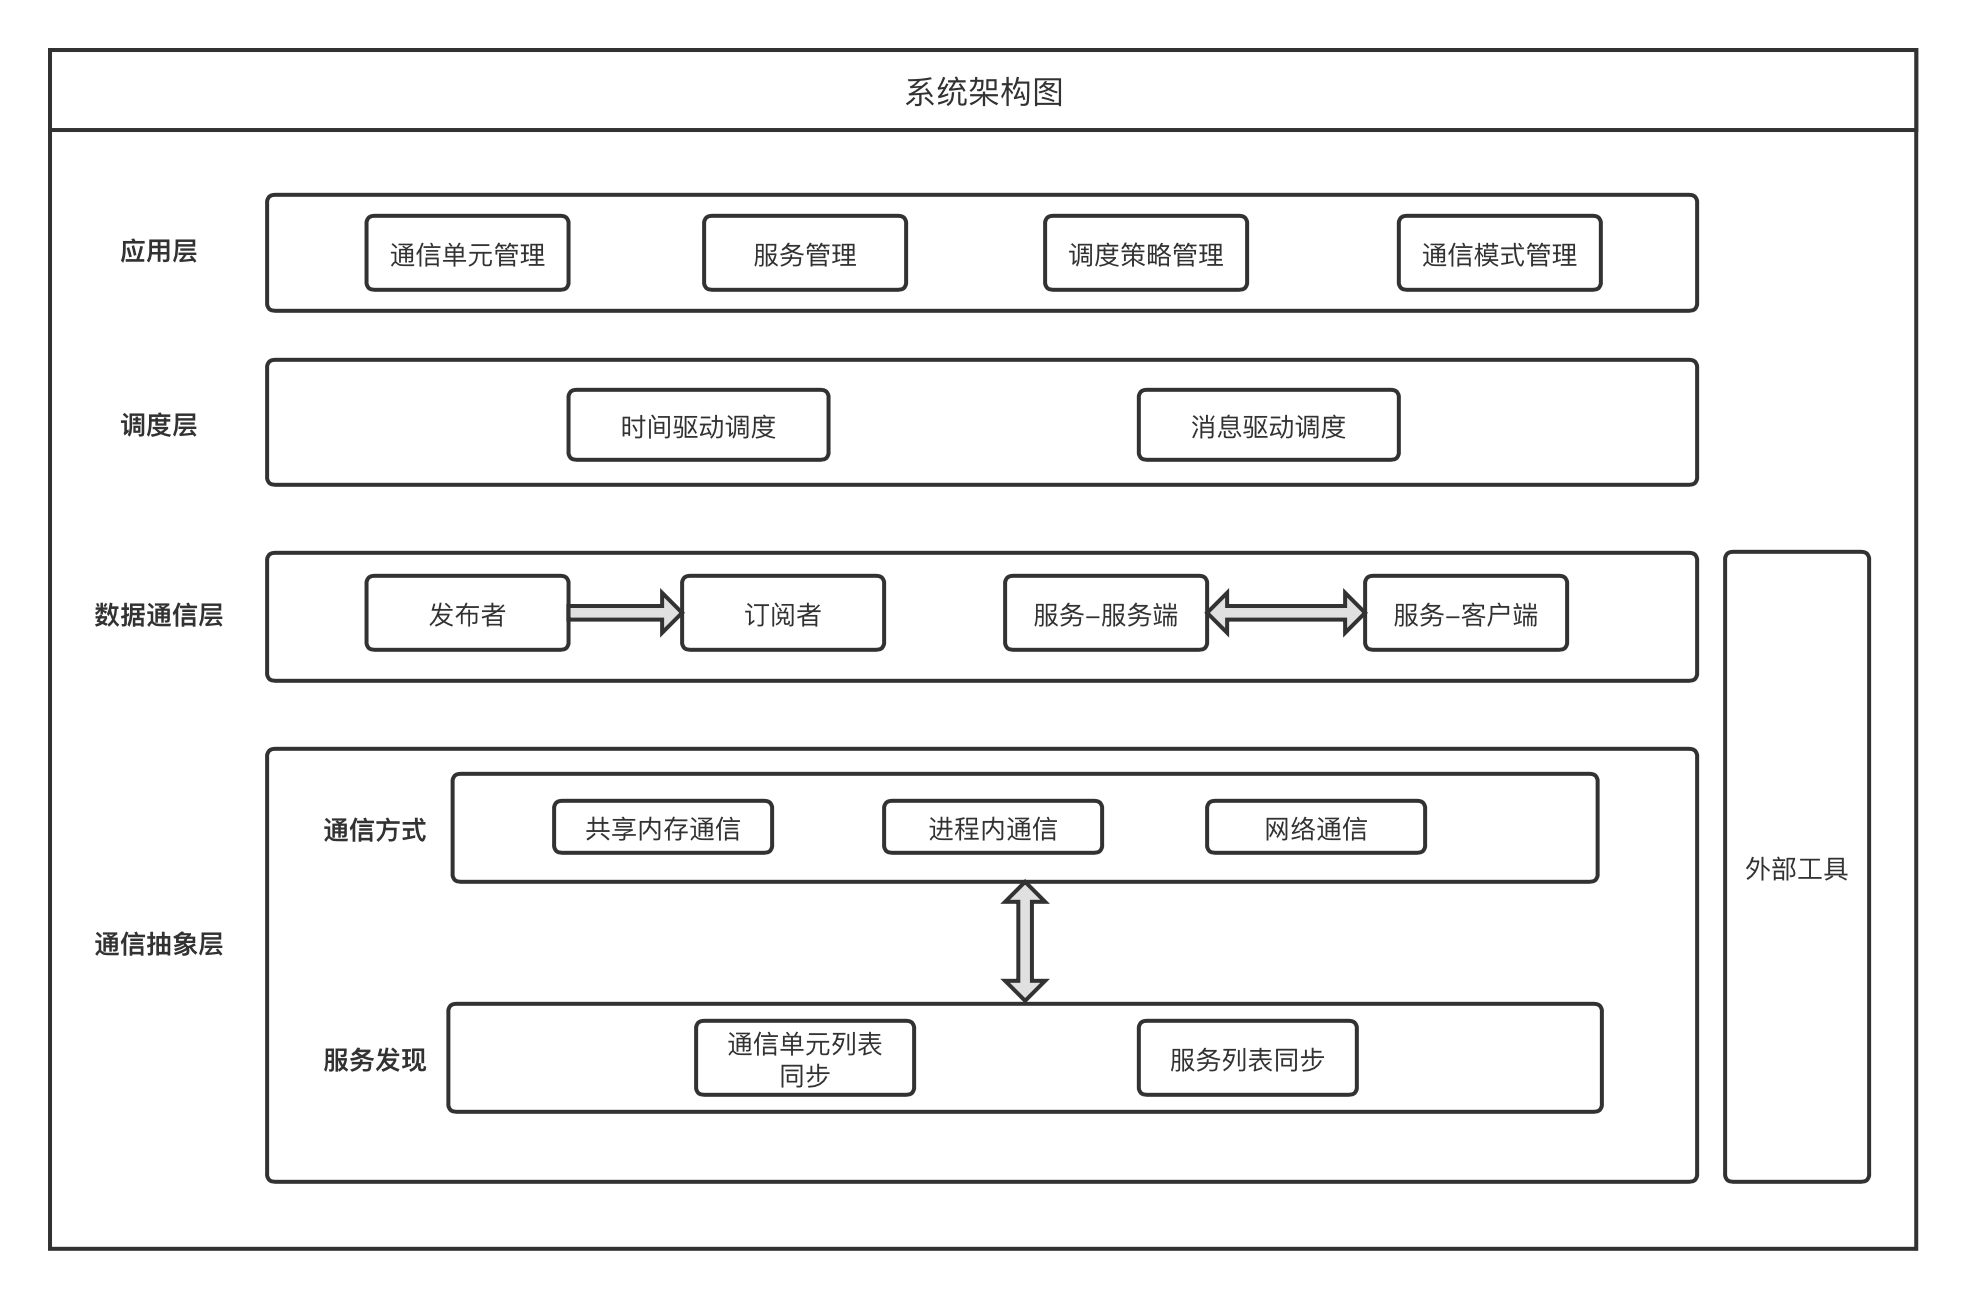
\includegraphics[width=1\textwidth]{4.1.png}
    \caption{自动驾驶运行时通信系统架构图}
    \label{communication_system_structure_gaiyao}
  \end{figure}

\subsection{通信系统组网设计}
针对通信系统网络拓扑动态变化的问题,如何使各分布在不同网络中的通信节点实时获取最新网络拓扑并相互发现
是最为关键的问题,即服务发现问题。本文对服务发现问题的解决方法是实现一个弱中心节点的方案,所有任务通过自身的服务发现模块
对中心节点发起RPC请求获取网络拓扑并完成通信的连接。弱中心节点的含义是中心节点只提供网络拓扑信息的查询与更新,并不参与
实际的通信。当任务内的通信单元或服务建立通信后消息通信是点对点的,不需要中心节点进行代理通信。

本文提出的自动驾驶运行时通信系统对于同一个局域网下的多个物理机不处于同一个网络中。本系统提供的通信域对通信范围作出了划分,
本机域指的是同一台物理机内的通信,全域指的是在网络内所有物理机之间的通信。本系统组网设计如图\ref{communication_system_network_gaiyao}所示。

\begin{figure}[htb]
  \centering
  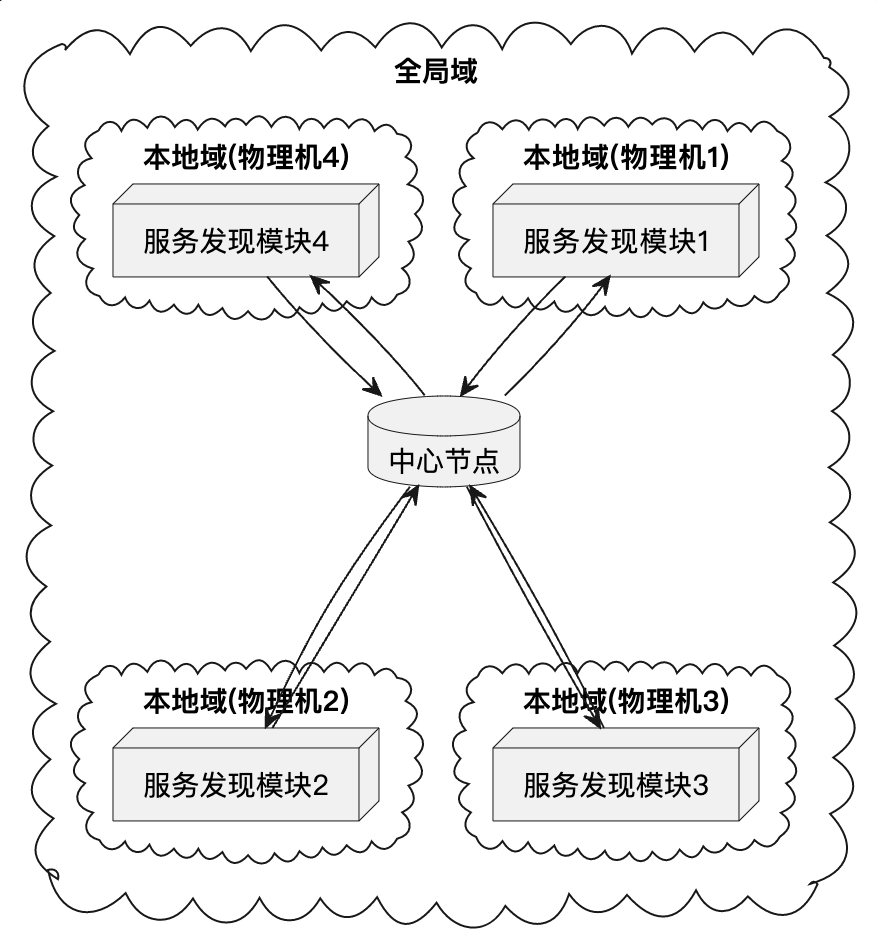
\includegraphics[width=0.5\textwidth]{4.2.png}
  \caption{通信系统组网设计图}
  \label{communication_system_network_gaiyao}
\end{figure}

\subsection{系统功能模块设计}
根据需求分析结果及系统架构,本文将系统分为如下七个模块:通信单元模块、服务模块、
任务模块、调度模块、通信传输模块、通信抽象模块及服务发现模块。本文根据业务与软件设计两个维度将系统模块层级分为一级模块与二级子模块,
其中通信单元模块、任务模块、通信传输模块与通信抽象模块被分为多个二级子模块,系统功能模块设计如图\ref{communication_system_function_module}所示。
根据功能模块图所示,本文设计的自动驾驶运行时通信系统各模块实现功能如下:
\begin{enumerate}
  \item 通信单元模块:包含发布者模块与订阅者模块两个二级子模块,该模块实现基于发布-订阅通信模式功能,同时
  向用户提供接口。发布者模块实现发布消息和管理发布者功能;订阅者模块实现订阅消息和管理订阅者功能。
  \item 服务模块:包含服务服务端和服务客户端两个二级子模块,该模块实现基于请求-响应的通信模式功能,同时向用户
  提供接口。服务服务端实现注册服务和管理服务端功能;服务客户端实现请求服务和管理客户端功能。
  \begin{figure}[htb]
    \centering
    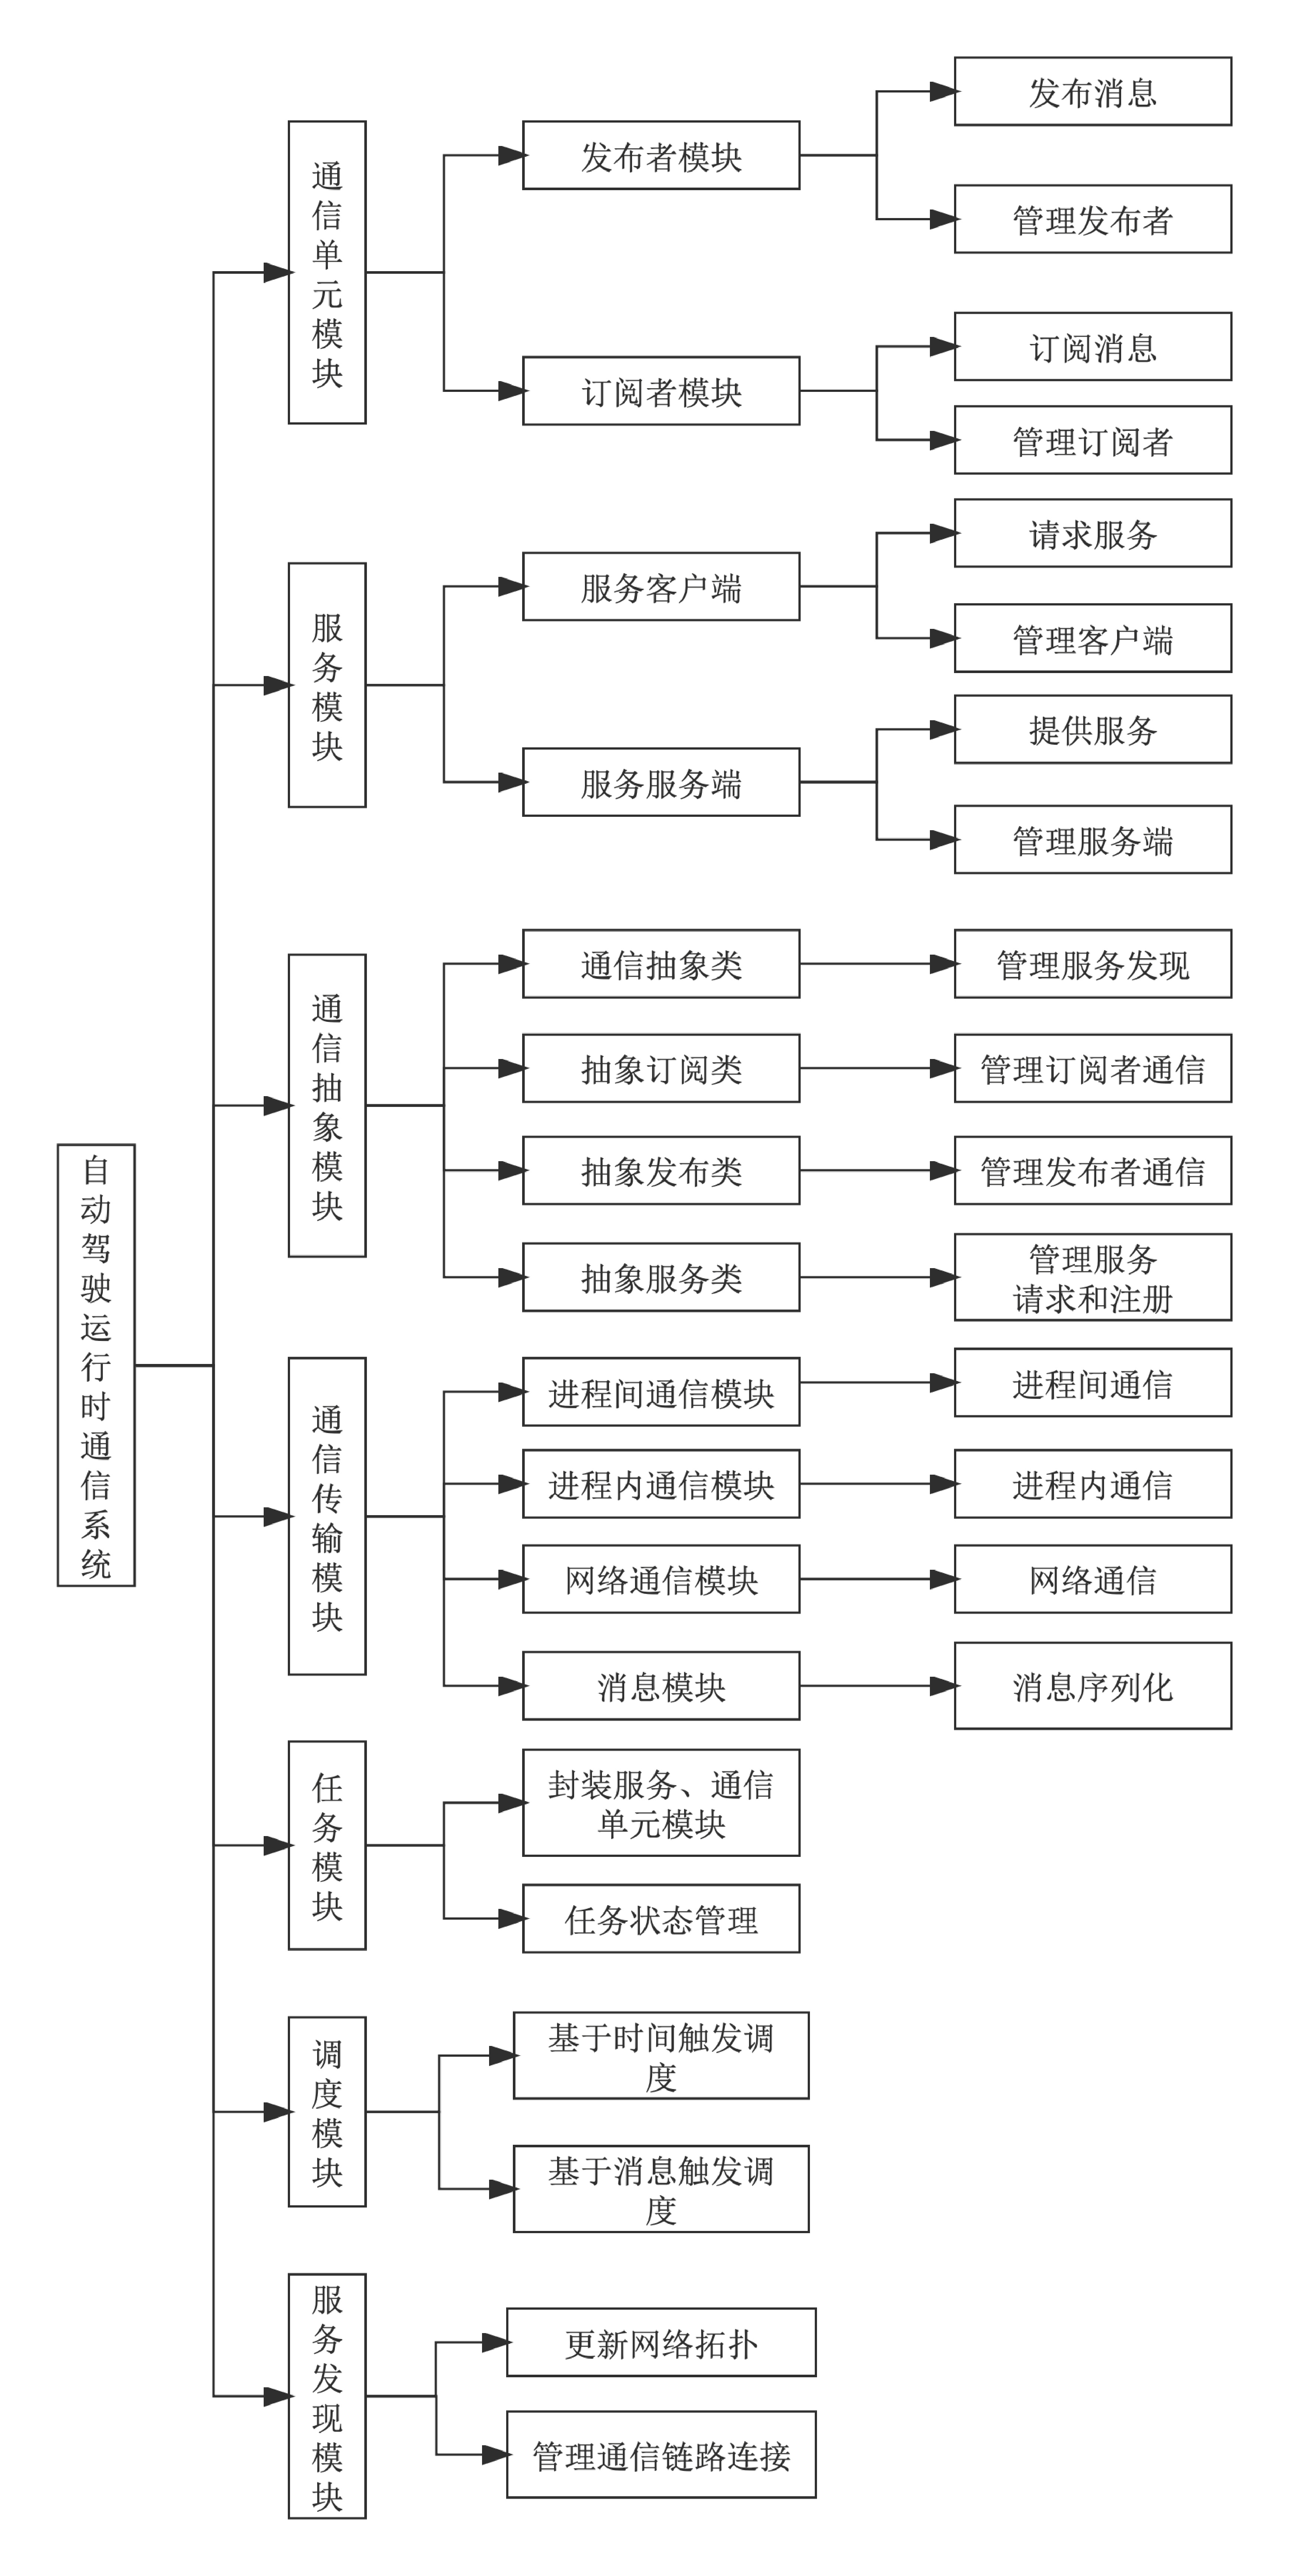
\includegraphics[width=0.6\textwidth]{communication_system_function_module.pdf}
    \caption{自动驾驶运行时通信系统功能模块图}
    \label{communication_system_function_module}
  \end{figure}
  \item 通信抽象模块:包含通信抽象类、抽象订阅类、抽象发布类和抽象服务类四个二级子模块,该模块将通信单元模块
  和服务模块所有的操作进行统一管理并且负责生成服务发现请求参数供服务发现模块完成服务发现功能。抽象订阅类
  根据用户对通信单元模块与服务模块的管理动态创建抽象订阅类、抽象发布类和抽象服务类,并生成服务发现请求参数
  至服务发现模块;抽象订阅类控制每个订阅者的通信链路,并通过通信传输模块监听通信链路中的消息;抽象发布类控制每个发布者的通信链路,
  并将待发布消息通过通信传输模块发送消息;抽象服务类控制所有服务端与客户端的注册服务和请求服务操作。
  \item 通信传输模块:包含进程间通信模块、进程内通信模块、网络通信模块与消息模块四个子模块,该模块是通信系统
  发布-订阅通信模式的实际传输模块,发布者发布消息与订阅者订阅消息全部由该模块负责序列化与传输。进程间通信模块
  通过共享内存方式传输消息;进程内通信模块通过指针方式传输信息;网络通信模块通过ZeroMQ传输消息;消息模块负责
  将进程间通信模块与网络通信模块待传输消息进行序列化处理。
  \item 任务模块:该模块将所有的发布者、订阅者、服务服务端和服务客户端及用户的逻辑代码封装为一个统一的任务,
  同时提供对任务状态的管理功能。
  \item 调度模块:该模块将用户的任务进行调度,调度策略分为基于消息触发的调度策略和基于时间的调度策略。
  \item 服务发现模块:该模块一方面接收本进程通信抽象类的服务发现参数向中心节点寻找通信匹配方并控制通信双方的通信链路建立;
  另一方面接收中心节点的更新通知,更改本进程内通信方的通信链路。
\end{enumerate}


% 本文根据业务与软件设计两个维度将系统模块分为一级模块与二级模块。
% 一级模块为:通信单元模块、服务模块、通信抽象模块、通信传输模块、任务模块、调度模块和服务模块共七个功能模块。在
% 一级模块下,分为功能进一步细化的二级模块。其中,通信单元模块分为发布者模块和订阅者模块两个子模块;服务模块分为
% 服务服务端和服务客户端两个子模块;通信抽象模块分为发布抽象模块、订阅抽象模块和服务抽象模块三个子模块;通信传输模块
% 分为进程间通信模块、进程内通信模块和网络通信模块三个子模块;任务模块分为通信单元模块和服务模块两个子模块。
% 表4.1简要描述了一级模块与二级模块的功能。
% \begin{table}[htb]
%   \caption{分布式通信系统功能模块描述}
%   \centering
%   \begin{tabular}{ccc}
%     \toprule
%     一级模块 & 二级模块 & 模块功能介绍\\
%     \midrule
%     \multirow{2}{*}{通信单元模块} & 发布者模块 & 提供管理发布者、发布数据等功能。 \\ & 订阅者模块 & 提供管理订阅者、接收数据等功能。 \\
%     \multirow{2}{*}{服务模块} & 服务服务端 & 提供管理服务端、处理请求等功能。 \\ & 服务客户端 & 提供管理客户端、发出请求等功能。 \\
%     \multirow{3}{*}{通信抽象模块} & 发布抽象模块 & 根据服务发现模块结果为发布者模块建立通信链路。 \\ & 订阅抽象模块 & 根据服务发现模块结果为订阅者模块建立通信链路。\\ & 服务抽象模块 & 处理服务请求和服务结果的发送和接收。\\
%     \multirow{3}{*}{通信传输模块} & 进程间通信模块 & 发送和接收进程间通信数据。 \\ & 进程内通信模块 & 发送和接收进程内通信数据。 \\ & 网络通信模块 & 发送和接收网络通信数据。 \\
%     \multirow{2}{*}{任务模块} & 通信单元模块 & 为任务提供基于发布-订阅的异步数据通信功能。 \\ & 服务模块 & 为任务提供基于RPC的同步数据通信功能。 \\
%     调度模块 & 无 & 按策略调度任务,控制任务的运行与停止\\
%     服务发现模块 & 无 & \makecell[c]{请求与更新通信网络拓扑,\\为通信抽象模块提供通信链路信息。} \\
%     \bottomrule
%   \end{tabular}
%   \label{tab:my_label}
% \end{table}

\section{通信单元模块概要设计}
自动驾驶运行时通信系统基于发布-订阅的异步通信功能依靠通信单元模块完成,通信单元模块由发布者模块与订阅者模块两个子模块共同完成
此功能。通信单元模块是最靠近用户的模块之一,用户将直接使用该模块提供的接口管理发布者与订阅者。该模块的设计思想是尽可能
屏蔽系统最底层的复杂实现而提供高度抽象且易用的接口给用户。
\subsection{订阅者模块概要设计}
订阅者模块用于实现基于发布-订阅模式异步通信中订阅者的基础功能,并向用户提供管理订阅者和订阅消息的功能接口。
订阅者模块的管理接口包括创建订阅者、删除订阅者与修改订阅者通信域,订阅消息由订阅者模块内部通过消息队列完成,用户无需
调用显式接口完成订阅消息的操作。

订阅者模块内部保存订阅者配置文件,该文件决定了订阅者需要订阅的话题以及通信域,配置文件如表\ref{subscriber_config_file}所示。
配置文件中,Topic与Domain需要由用户显式给定,字段不可为空;QueueSize系统默认为100,用户可以自由设置消息队列的长度;
DataCallback为订阅者模块收到消息后执行的回调函数,系统默认的回调函数为将收到的消息压入消息队列,但用户可以自定义
收到消息后的回调函数。
\begin{table}[htb]
  \centering\small
  \caption{订阅者模块配置文件}
  \renewcommand\arraystretch{1.2}
  \label{subscriber_config_file}
  \begin{tabular}{cc}
    \toprule
    字段名 & 字段解释 \\
    \midrule
    Topic & 订阅者订阅消息的话题名称\\
    Domain & 订阅者所在的通信域\\
    QueueSize & 订阅者内部消息队列长度\\
    DataCallback & 订阅者接收到消息后执行的回调函数\\
    \bottomrule
  \end{tabular}
\end{table}

订阅者模块中的管理接口由用户直接调用,接口设计如表\ref{subscriber_interface}所示。管理接口中,create\_subscriber接口需要配置文件作为
参数并根据话题名称与通信域供服务发现模块进行服务发现并与匹配的发布者进行点对点的连接;delete\_subscriber接口
需要由用户指定删除类型,接口内部根据删除类型判断是否需要保存未接受的消息并向服务发现模块发出删除请求;modify\_subscriber\_domain接口需要由用户指定修改
后的通信域作为参数;query\_publishers\_info与query\_subscribers\_info接口根据查询范围与查询条件查询系统内的发布者信息或订阅者信息,
查询范围可以选择本地域或全域,查询条件可以选择按话题查询或全量查询。
\begin{table}[htb]
  \renewcommand\arraystretch{1.2}
  \centering\small
  \caption{订阅者模块接口}
  \label{subscriber_interface}
  \begin{tabular}{cc}
    \toprule
    接口签名 & 接口解释 \\
    \midrule
    create\_subscriber & 创建订阅者\\
    delete\_subscriber & 删除订阅者\\
    modify\_subscriber\_domain & 修改订阅者通信域\\
    query\_publishers\_info & 查询发布者信息\\
    query\_subscribers\_info & 查询订阅者信息\\
    \bottomrule
  \end{tabular}
\end{table}


订阅者模块中的消息队列保存自身订阅话题对应发布者发布的消息,根据消息队列大小动态地接收与丢弃消息队列中
保存的消息。消息队列在基于C++标准库提供的队列之上加入了互斥锁与条件变量以保证消息同步性。同样地,消息队列
也向用户提供了操作接口,接口设计如表\ref{message_queue_interface}所示。

% \begin{table}[H]
%   \centering\small
%   \caption{消息队列相关接口}
%   \label{tab:exampletable}
%   \begin{tabular}{cc}
%     \toprule
%     接口签名 & 接口解释 \\
%     \midrule
%     size & 查询队列中消息的数量\\
%     empty & 查询队列是否为空\\
%     pop & 从队列的队头取出一条消息\\
%     pop\_newest & 从队列取出最新消息,即从队列的队尾取出一条消息\\
%     pop\_newest\_and\_clear & 从队列取出最新消息并清空队列中所有消息\\
%     \bottomrule
%   \end{tabular}
% \end{table}
\begin{longtable}{cc}
  \caption{消息队列相关接口}\label{message_queue_interface}\\
  % 表格“首页”显示内容
  \toprule
  接口签名 & 接口解释 \\
  \midrule
  \endfirsthead
  % “后续页面”表头显示内容
  \multicolumn{2}{r}{续表4.3}\\
  \toprule
  接口签名 & 接口解释 \\
  \hline
  %\midrule
  \endhead
  % 表格“尾页前”,表格最后显示内容
  %\bottomrule
  \endfoot
  % 表格“尾页”,表格最后显示内容
  \bottomrule
  \endlastfoot

  size & 查询队列中消息的数量\\
  empty & 查询队列是否为空\\
  pop & 从队列的队头取出一条消息\\
  pop\_newest & 从队列取出最新消息,即从队列的队尾取出一条消息\\
  pop\_newest\_and\_clear & 从队列取出最新消息并清空队列中所有消息\\
  \end{longtable}  

订阅者模块的时序设计如图\ref{subscriber_gaiyao_timesequence}所示。
用户调用创建订阅者接口后,订阅者模块首先校验配置文件中的必填字段是按要求填写,若配置文件校验失败则本次创建失败;
配置文件校验成功后,将其中的回调函数作为任务调度模块的调度任务;调度任务设置完成后,将配置文件传至通信抽象模块,
通信抽象模块根据配置文件信息创建抽象订阅类,在订阅者配置文件的基础上加入IP地址、进程号以及订阅者更新通信链路的回调函数
形成抽象订阅者配置文件,作为服务发现参数传至服务发现模块;服务模块根据抽象订阅者配置文件中的IP地址、进程号、话题名称以及通信域
进入循环寻找与订阅者匹配的发布者,若寻找成功则调用抽象订阅者配置文件中的回调函数,发布订阅双方完成点对点的连接并开始通信。
\begin{figure}[H]
  \centering
  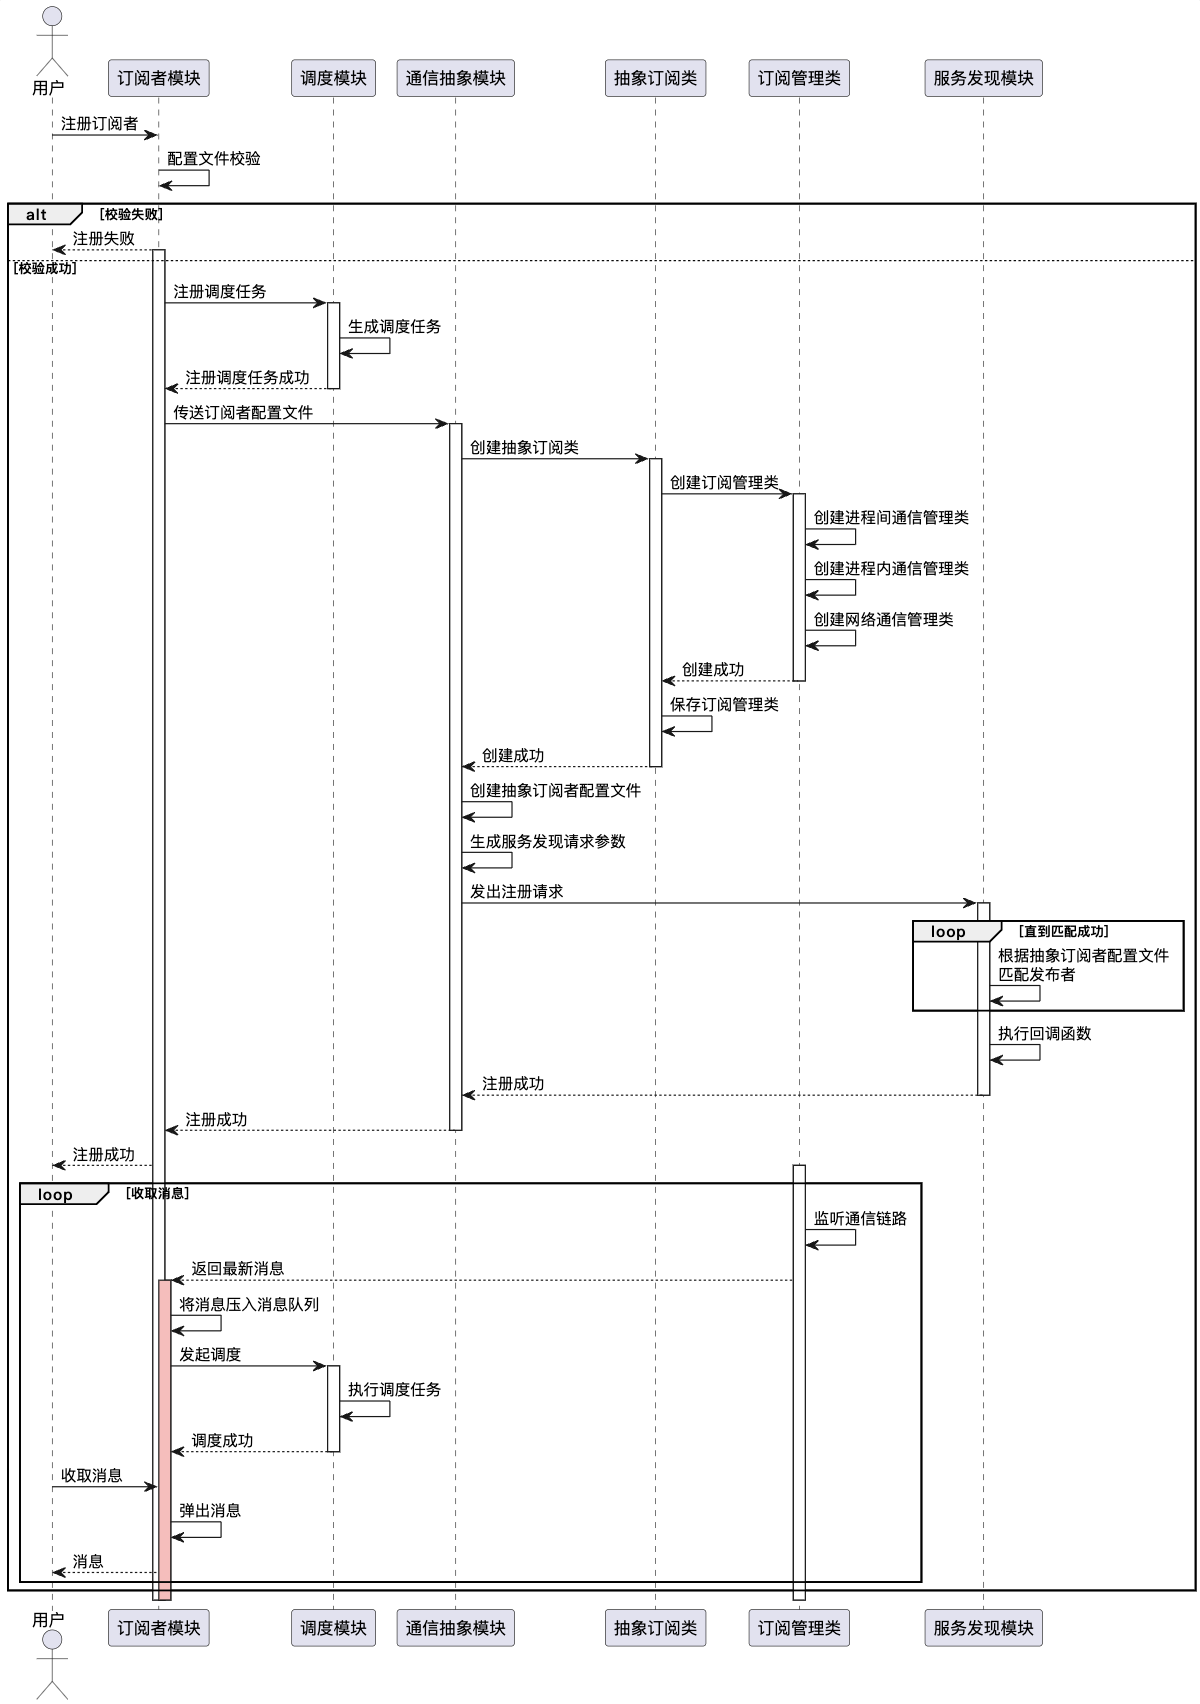
\includegraphics[width=0.85\textwidth]{subscriber_gaiyao_timesequence.png}
  \caption{创建订阅者时序图}
  \label{subscriber_gaiyao_timesequence}
\end{figure}

% \begin{figure}[H]
%   \centering
%   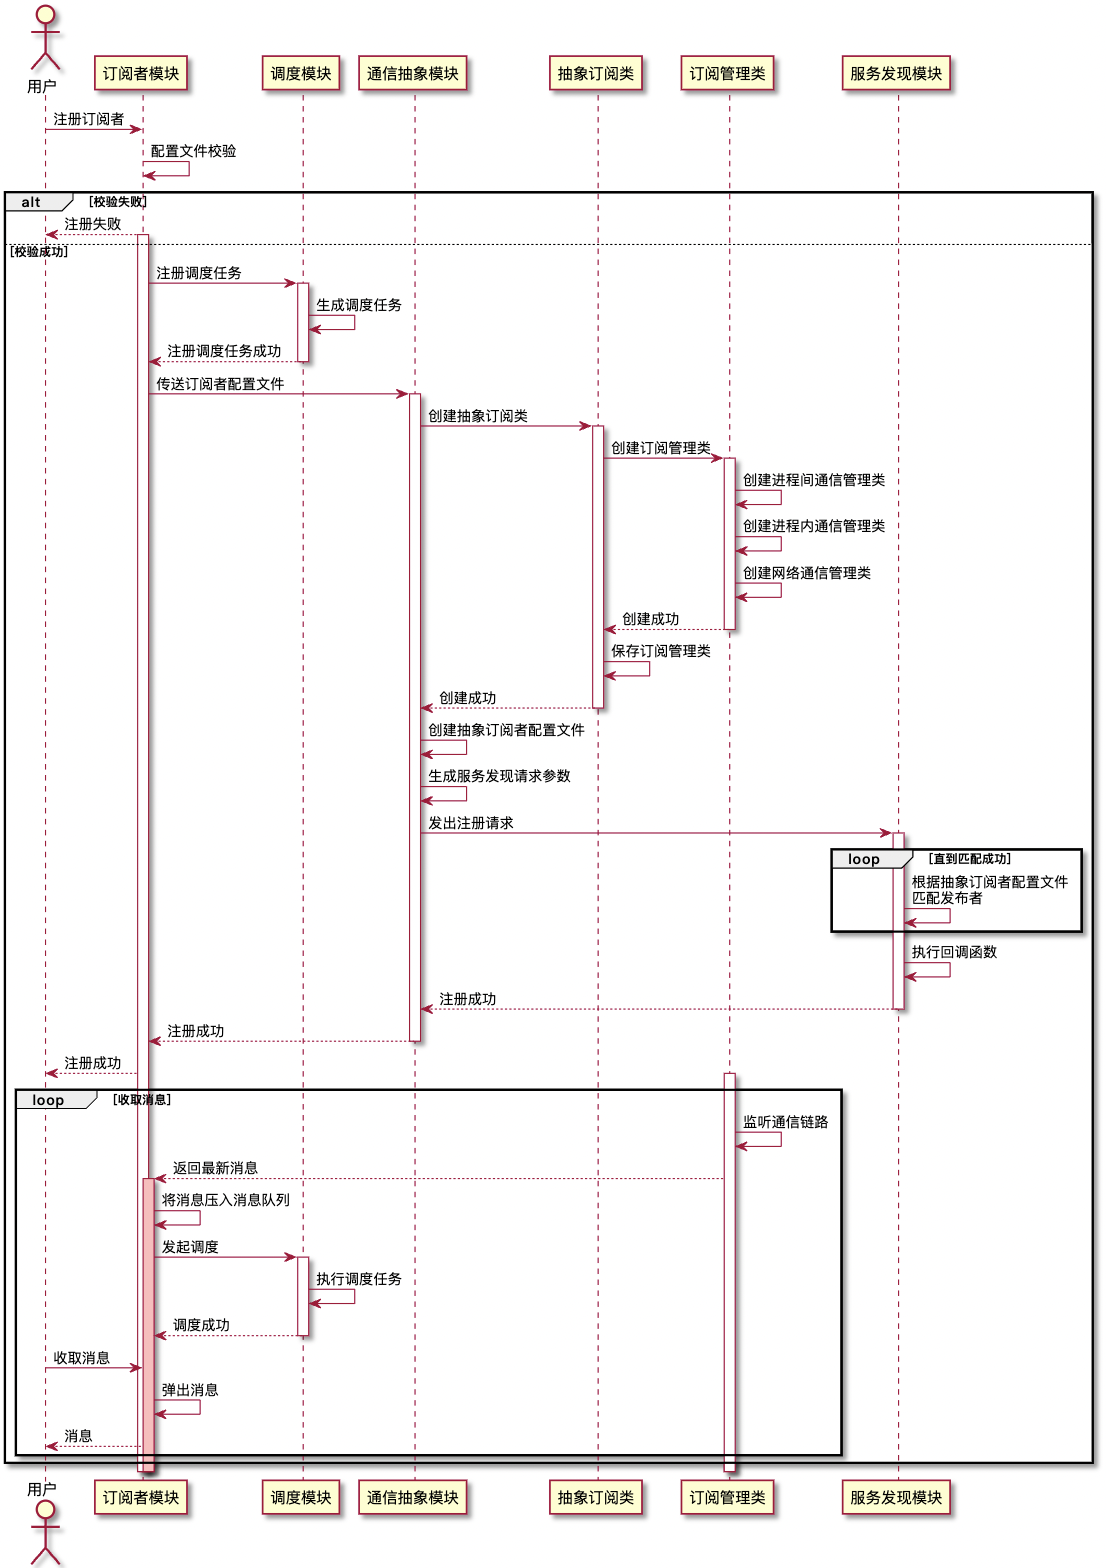
\includegraphics[width=0.8\textwidth]{4.4.png}
%   \caption{创建订阅者时序图}
%   \label{fig:24}
% \end{figure}

\subsection{发布者模块概要设计}
发布者模块用于实现基于发布-订阅模式异步通信中发布者的基础功能,并向用户管理订阅者和发布消息的功能接口。
发布者模块的管理接口包括创建发布者、删除发布者与修改发布者通信域,发布消息接口由发布者模块唯一提供。

同订阅者模块类似,发布者模块内部保存了发布者配置文件,该文件决定了发布者发布消息的话题以及通信域,配置文件如表\ref{publisher_config_file}所示。
由于发布者内部并不需要维护消息队列,其配置文件内容相比订阅者配置文件较少,但Topic与Domain仍需要由用户显式给定。
\begin{table}[htb]
  \centering\small
  \caption{发布者模块配置文件}
  \renewcommand\arraystretch{1.2}
  \label{publisher_config_file}
  \begin{tabular}{cc}
    \toprule
    字段名 & 字段解释 \\
    \midrule
    Topic & 发布者发布消息的话题名称\\
    Domain & 发布者所在的通信域\\
    \bottomrule
  \end{tabular}
\end{table}

发布者模块中的管理接口和发布消息接口由用户直接调用,接口设计如表\ref{publisher_interface}所示。同订阅者模块的管理接口类似,create\_publisher
需要配置文件作为参数并根据配置文件中的话题名称与通信域供服务发现模块寻找匹配的订阅者进行点对点连接;delete\_publisher
接口同样不需要任何参数,由接口内部向服务发现模块发出删除请求;modify\_publisher\_domain接口需要由用户指定修改后的
通信域作为参数;publish接口是发布者发布消息的唯一接口;query\_publishers\_info与query\_subscribers\_info接口功能与订阅者模块中的接口功能相同。
\begin{table}[htb]
  \centering\small
  \renewcommand\arraystretch{1.2}
  \caption{发布者模块接口}
  \label{publisher_interface}
  \begin{tabular}{cc}
    \toprule
    接口签名 & 接口解释 \\
    \midrule
    create\_publisher & 创建发布者\\
    delete\_publisher & 删除发布者\\
    modify\_publisher\_domain & 修改发布者通信域\\
    publish & 发布消息 \\
    query\_publishers\_info & 查询发布者信息\\
    query\_subscribers\_info & 查询订阅者信息\\
    \bottomrule
  \end{tabular}
\end{table}

发布者模块的创建、删除与修改流程与订阅者模块大致相似,二者不同的地方是通信抽象模块会返回与该发布者对应的抽象发布类,
发布者模块保存该类并通过该类中保存的发布管理类进行发布消息;创建发布者过程中不需要向调度模块注册调度任务。
发布者创建及发布消息时序设计如图\ref{publisher_gaiyao_timesequence}所示。

\begin{figure}[H]
  \centering
  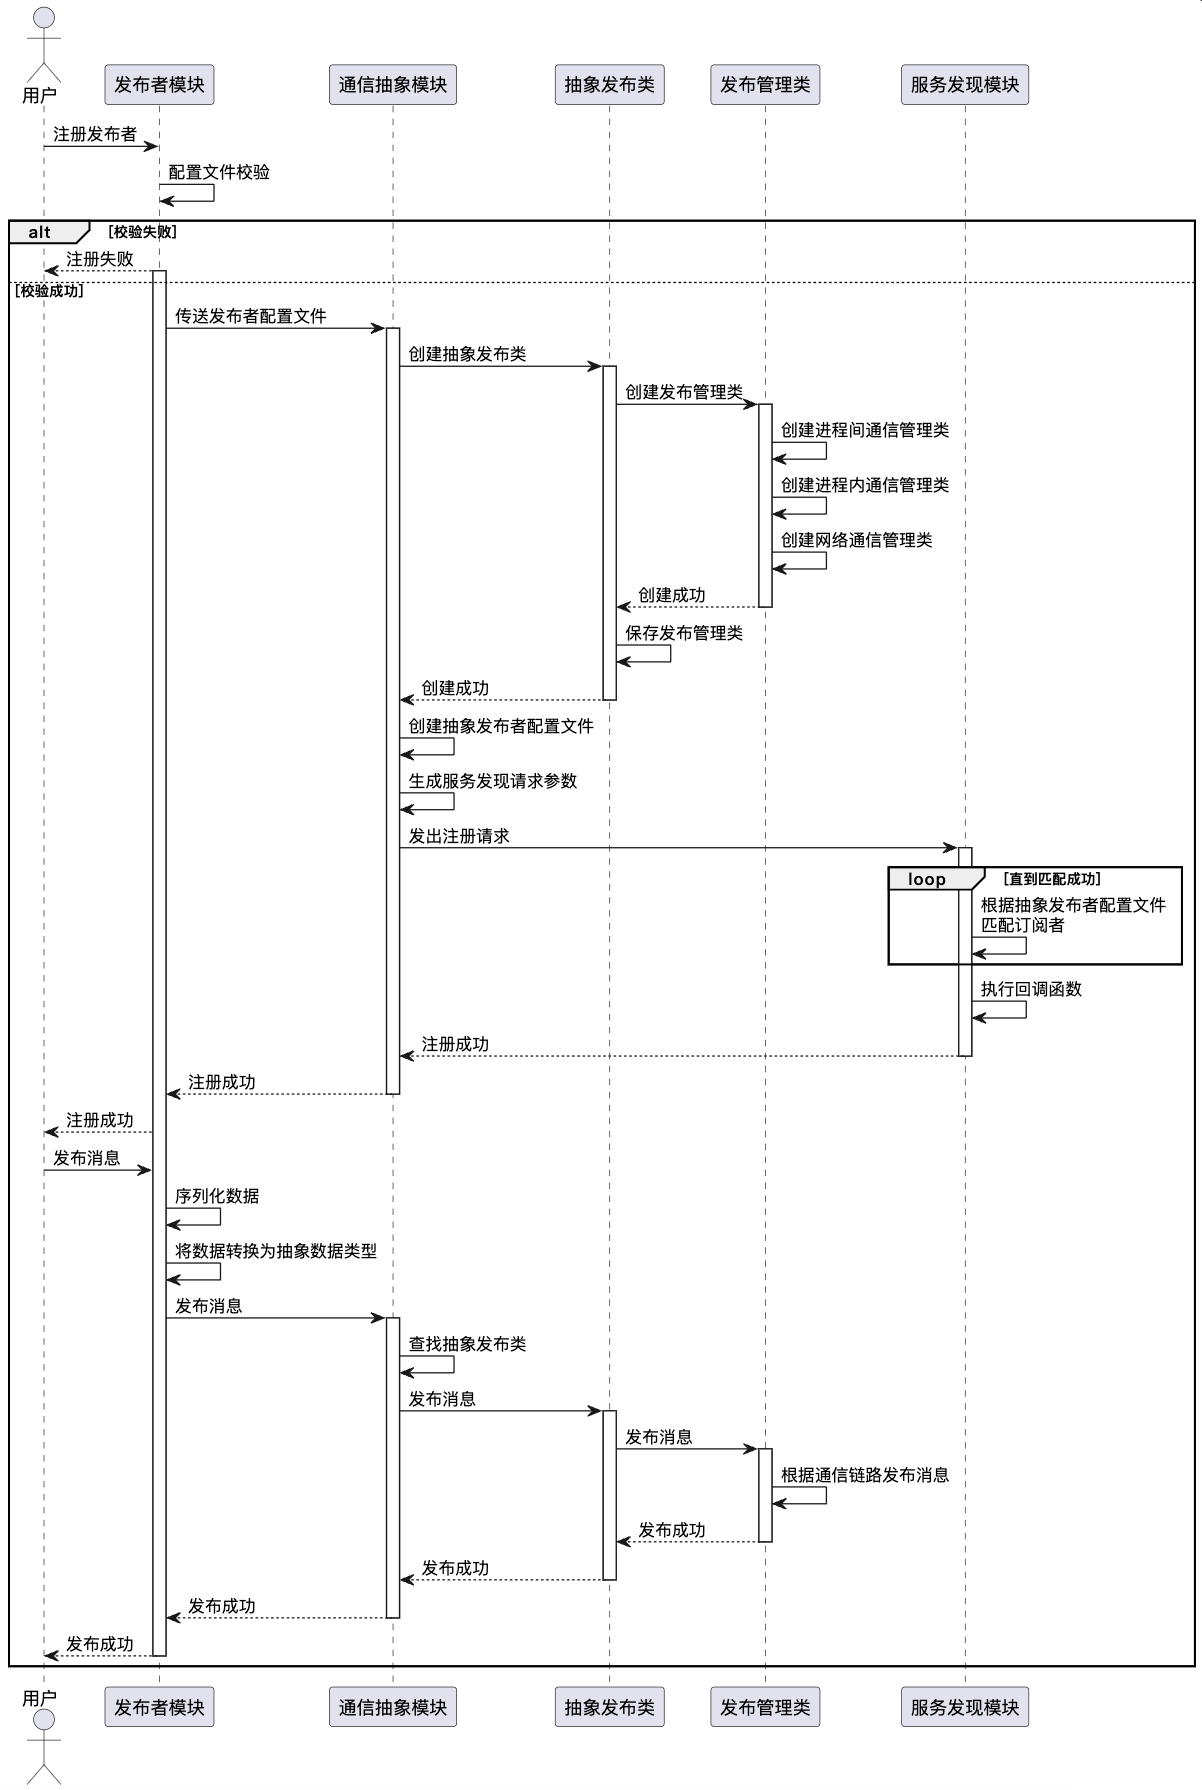
\includegraphics[width=0.8\textwidth]{publisher_gaiyao_timesequence.png}
  \caption{创建发布者时序图}
  \label{publisher_gaiyao_timesequence}
\end{figure}

\section{服务模块概要设计}
自动驾驶运行时通信系统基于RPC的同步数据通信功能由服务模块实现,服务模块功能由服务服务端与服务客户端两个子模块共同完成。

\subsection{服务客户端设计}
服务客户端用于实现基于RPC同步数据通信中客户端即服务请求方的基础功能,提供管理服务客户端接口及请求服务的功能接口。

服务客户端内部保存客户端配置文件,该文件决定了客户端需要请求的服务名称、通信域,配置文件如表\ref{service_client_config_file}所示。
配置文件中,ServiceName与Domain需要由显式给定,不可为空。
\begin{table}[H]
  \centering\small
  \caption{服务客户端配置文件}
  \label{service_client_config_file}
  \renewcommand\arraystretch{1.2}
  \begin{tabular}{cc}
    \toprule
    字段名 & 字段解释 \\
    \midrule
    ServiceName & 服务客户端需要调用服务的名称\\
    Domain & 服务客户端请求服务的通信域范围\\
    \bottomrule
  \end{tabular}
\end{table}

服务客户端接口设计如表\ref{service_client_interface}所示。create\_service\_client根据客户端配置文件中的ServiceName与Domain初始化服务客户端;
delete\_service\_client不需要任何参数,被调用后直接删除客户端,删除过程不需要由服务发现模块参与;
modify\_service\_client\_domain在接收用户指定的目标通信域后由服务发现模块完成通信域的切换;
is\_service\_available接口实现查询客户端需要请求服务可用性;call\_service接口实现发起向服务服务端发起请求;
query\_service\_list接口根据查询范围与查询条件查询系统内现有服务列表,查询范围可以选择本地域或全域,查询条件可以选择按服务名称查询或全量查询。
\begin{table}[htb]
  \centering\small
  \caption{服务客户端接口}
  \renewcommand\arraystretch{1.2}
  \label{service_client_interface}
  \begin{tabular}{cc}
    \toprule
    接口签名 & 接口解释 \\
    \midrule
    create\_service\_client & 创建服务客户端\\
    delete\_service\_client & 删除服务客户端\\
    modify\_service\_client\_domain & 修改服务客户端通信域\\
    is\_service\_available & 查询服务可用性 \\
    call\_service & 发起服务请求\\
    query\_service\_list & 查询现有服务列表\\
    \bottomrule
  \end{tabular}
\end{table}

服务客户端的创建、删除与修改通信域与通信单元模块中的订阅者模块流程有较大区别,服务客户端的信息并不需服务发现模块
更新至通信网络拓扑中,只需要服务模块帮助查询对应服务的服务端IP地址即可由RPC完成通信。

用户调用创建服务客户端接口后,服务客户端保存配置文件并将配置文件并将配置文件作为参数传至通信抽象模块;
通信抽象模块根据配置文件字段创建抽象服务类作为实际发起RPC调用的辅助类,创建完成后将配置文件传至服务发现模块;
服务发现模块将配置文件保存即结束创建工作,服务客户端保存抽象服务类实例后向用户返回创建成功信息。

用户调用发起服务请求接口后,服务客户端通过调用保存的抽象服务类发起实际的RPC调用,调用完成后向用户返回结果。
服务客户端的时序设计如图\ref{client_gaiyao_timesequence}所示。

\begin{figure}[H]
  \centering
  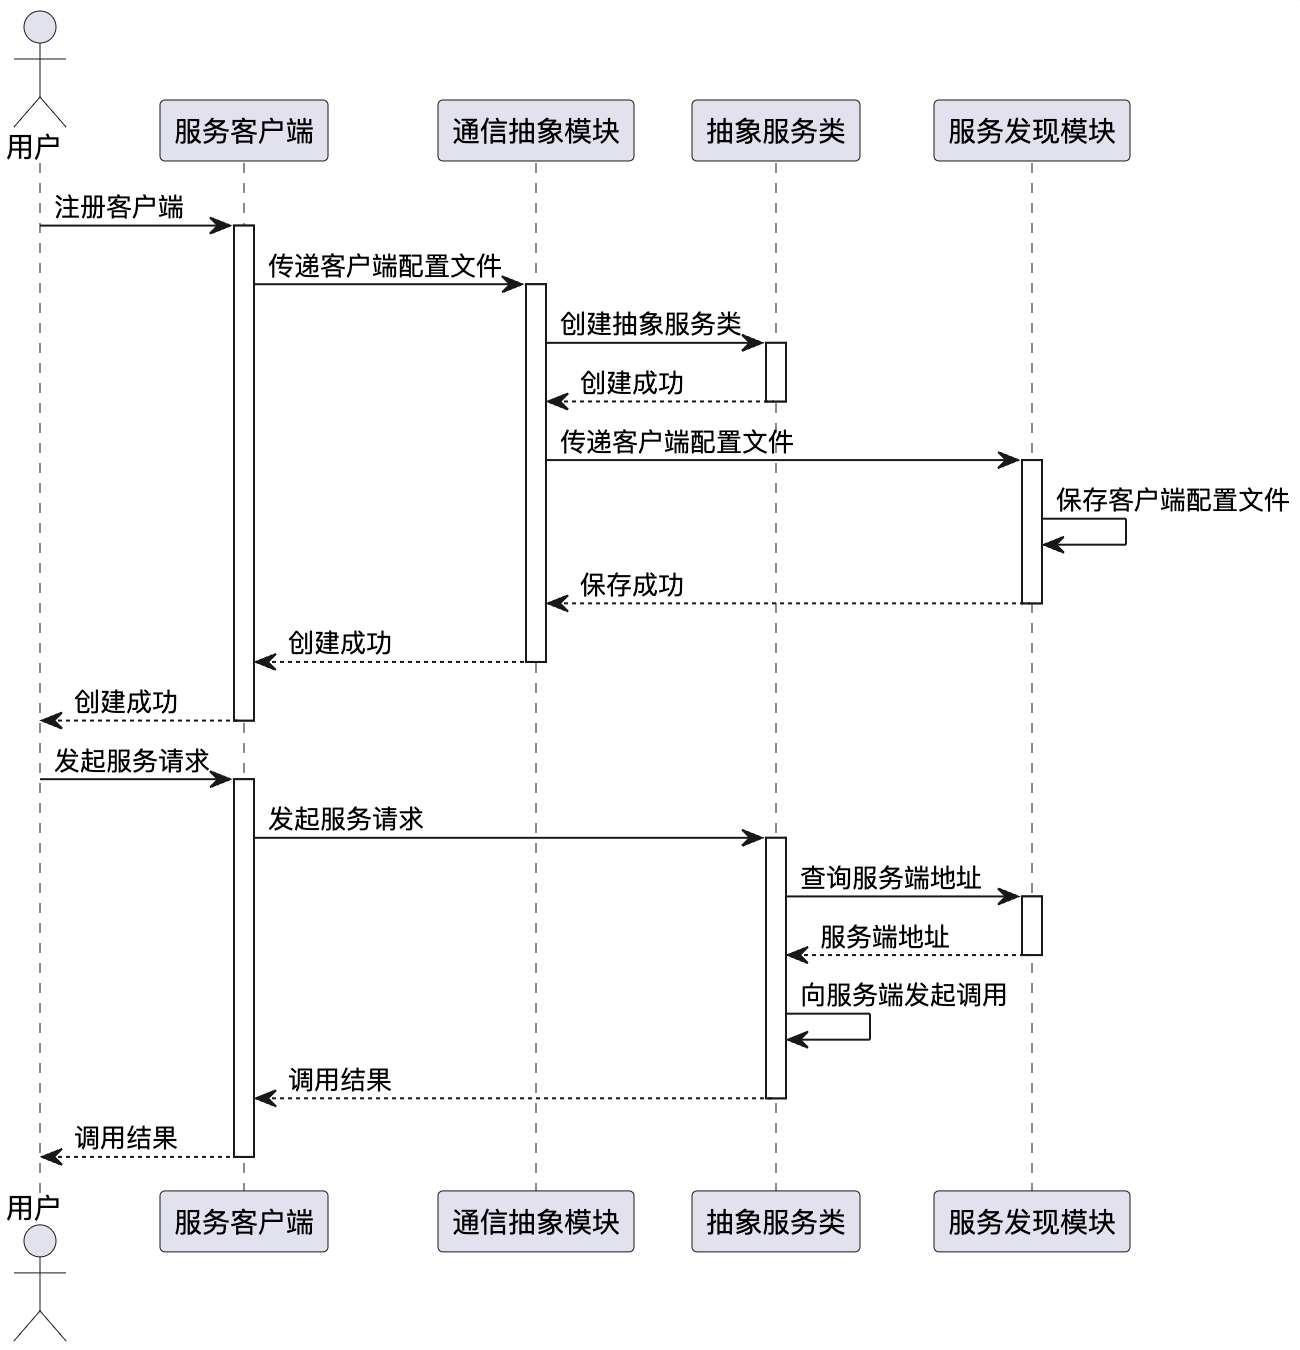
\includegraphics[width=0.85\textwidth]{client_gaiyao_timesequence.png}
  \caption{服务客户端时序图}
  \label{client_gaiyao_timesequence}
\end{figure}

\subsection{服务服务端设计}
服务服务端用于实现基于RPC同步数据通信中服务端即服务提供方的基础功能,提供管理服务端接口及创建服务的功能接口。

服务服务端内部保存服务端配置文件,该文件决定了服务端提供的服务名称、服务功能以及通信域,配置文件如表\ref{service_server_config_file}所示。
配置文件中的所有字段全部由用户显式给定,不能为空。
\begin{table}[H]
  \centering\small
  \caption{服务服务端配置文件}
  \renewcommand\arraystretch{1.05}
  \label{service_server_config_file}
  \begin{tabular}{cc}
    \toprule
    字段名 & 字段解释 \\
    \midrule
    ServiceName & 服务客户端需要调用服务的名称。\\
    Domain & 服务客户端请求服务的通信域范围。\\
    ServiceCallback & 服务端提供的处理函数。\\
    \bottomrule
  \end{tabular}
\end{table}

服务服务端接口设计如表\ref{service_server_interface}所示。服务服务端提供的接口与服务客户端大致相同。根据服务端的特点,服务端接口
删除了客户端中的发起服务请求接口与查询服务可用性接口。
\begin{table}[htb]
  \centering\small
  \caption{服务服务端接口}
  \renewcommand\arraystretch{1.2}
  \label{service_server_interface}
  \begin{tabular}{cc}
    \toprule
    接口签名 & 接口解释 \\
    \midrule
    create\_service\_server & 创建服务端 \\
    delete\_service\_server & 删除服务端\\
    modify\_service\_server & 修改服务端通信域\\
    query\_service\_list & 查询现有服务列表\\
    \bottomrule
  \end{tabular}
\end{table}

不同于服务客户端,服务端的创建、删除、修改需要服务发现模块参与更新网络拓扑。

\begin{figure}[H]
  \centering
  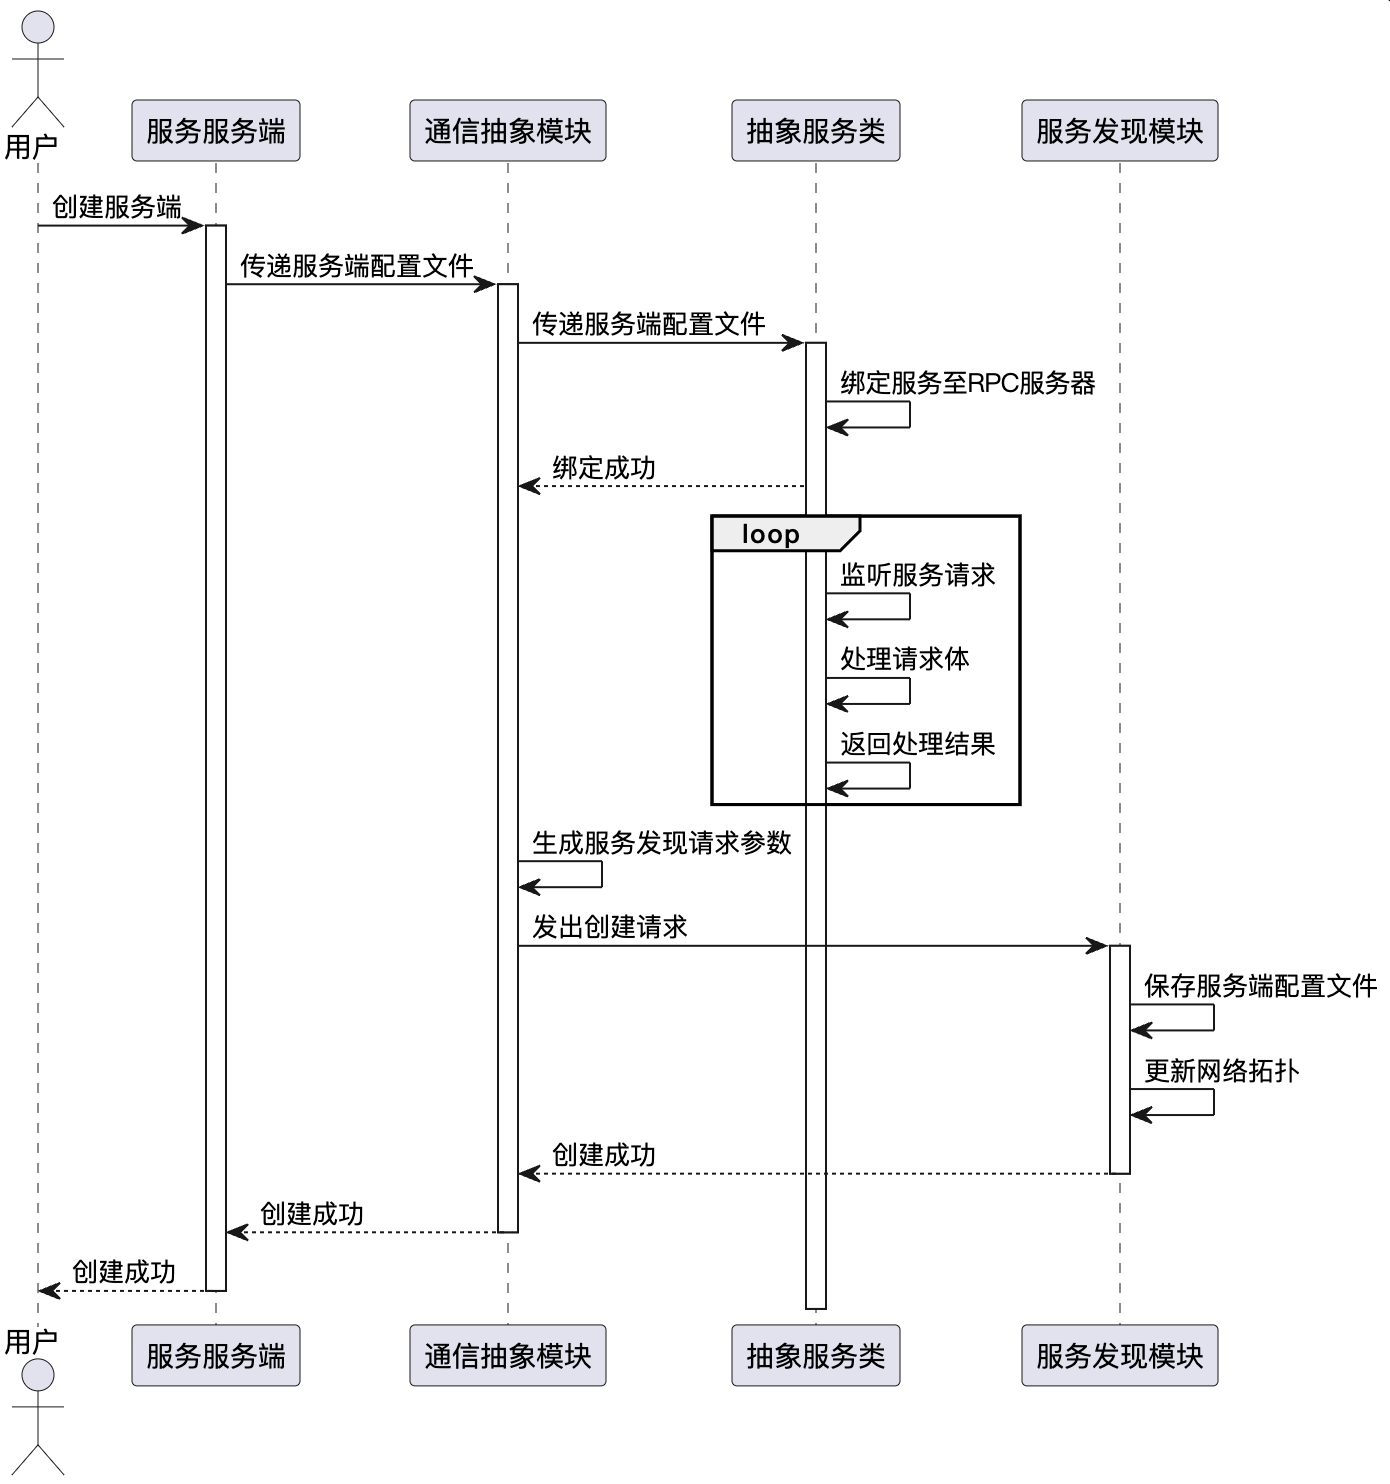
\includegraphics[width=0.8\textwidth]{server_gaiyao_timesequence.png}
  \caption{服务服务端时序图}
  \label{server_gaiyao_timesequence}
\end{figure}

服务服务端时序设计如图\ref{server_gaiyao_timesequence}所示。用户调用创建创建服务端接口后,服务端保存配置文件并将配置文件作为参数传至通信抽象模块;通信抽象模块
将配置文件作为参数传至抽象服务类,抽象服务类根据配置文件绑定服务至本地RPC服务器中;通信抽象模块
在配置文件基础上添加IP地址和端口号并作为服务发现请求参数传至服务发现模块;服务发现模块根据请求参数更新网络拓扑,
随后向用户返回创建成功信息;服务端创建成功后,由服务抽象类负责监听服务请求并根据用户提供的回调函数对
请求体进行处理.


\section{通信抽象模块概要设计}
通信抽象模块是整个自动驾驶运行时通信系统中最为重要的模块之一,
该模块将通信单元和服务的所有操作如创建、删除、修改、发布消息等在通信抽象类中进行统一管理,
并负责创建抽象发布类、抽象订阅类与抽象服务类完成消息的发布-订阅功能与服务的请求-应答功能。
此外,该模块将发布者、订阅者、服务服务端与服务客户端的信息同步至服务发现模块完成服务发现功能。


\subsection{通信抽象类概要设计}
通信抽象类负责处理通信单元模块和服务模块的所有请求,控制抽象发布类、抽象订阅类与抽象服务类的创建与删除,协助
服务发现模块完成服务发现功能,该类唯一存在,其接口设计如表\ref{communication_abstract_interface}所示。
 
\begin{table}[htb]
  \centering\small
  \caption{通信抽象模块接口}
  \renewcommand\arraystretch{1.2}
  \label{communication_abstract_interface}
  \begin{tabular}{cc}
    \toprule
    接口签名 & 接口解释 \\
    \midrule
    create\_publisher & 处理创建发布者请求\\
    delete\_publisher & 处理删除发布者请求\\
    modify\_publisher\_domain & 处理发布者更改通信域请求\\
    publish & 处理发布者发布消息请求 \\
    create\_subscriber & 处理创建订阅者请求\\
    delete\_subscriber & 处理删除订阅者请求\\
    modify\_subscriber\_domain & 处理订阅者更改通信域请求\\ 
    create\_service\_server & 处理创建服务服务端请求\\
    delete\_service\_server & 处理删除服务服务端请求\\
    modify\_service\_server\_domain & 处理修改服务服务端通信域请求\\
    create\_service\_client & 处理创建服务客户端请求\\
    delete\_service\_client & 处理删除服务客户端请求\\
    modify\_service\_client\_domain & 处理修改服务客户端通信域请求\\
    query\_subscribers\_info & 查询系统内订阅者信息\\
    query\_publishers\_info & 查询系统内发布者信息\\
    query\_service\_server\_info & 查询系统内服务端信息\\
    \bottomrule
  \end{tabular}
\end{table}

通信抽象类在处理发布者或订阅者的创建请求时,会生成与其对应的抽象发布类或抽象订阅类,并在类中为其绑定更新
通信链路的回调函数供服务发现模块收到网络拓扑变化时调用,并在配置文件的基础上加入本机IP地址以及本进程的进程号生成
服务发现请求参数。
处理服务端或客户端的创建请求时,会创建抽象服务类并由该类完成基于RPC的通信功能,并不需要
在抽象服务类中绑定更新通信链路的回调函数。通信抽象类在服务端的配置文件基础上加入本机IP地址,而对客户端的配置文件
不加入任何信息,随后生成对应服务发现请求参数。服务发现请求参数如表\ref{service_discovery_parameter}所示。

\begin{table}[htb]
  \centering\small
  \caption{服务发现请求参数}
  \renewcommand\arraystretch{1.12}
  \label{service_discovery_parameter}
  \begin{tabular}{ccc}
    \toprule
    接口签名 & 接口解释 \\
    \midrule
    \multirow{4}{*}{PublisherInfo} & Topic & 发布者发布消息的话题名称 \\ & Domain & 发布者所在的通信域 \\ & Address & 发布者的IP地址和进程号 \\ & Callback & \makecell[c]{根据订阅者信息更新通信链路的回调函数}\\
    \cline{2-3}
    \multirow{4}{*}{SubscriberInfo} & Topic & 订阅者订阅消息的话题名称 \\ & Domain & 订阅者所在的通信域 \\ & Address & 订阅者的IP地址和进程号 \\ & Callback & \makecell[c]{根据发布者信息更新通信链路的回调函数}\\
    \cline{2-3}
    \multirow{4}{*}{ServiceServerInfo} & ServiceName & 服务端提供服务的名称 \\ & Domain & 服务端提供服务的通信域 \\ & IP & 服务端的IP地址 \\ & port & 服务端的端口\\
    \cline{2-3}
    \multirow{2}{*}{ServiceClientInfo} & ServiceName & 客户端请求服务的名称 \\ & Domain & 客户端请求服务的通信域 \\
    \bottomrule
  \end{tabular}
\end{table}

\subsection{抽象发布类概要设计}
抽象发布类内部创建通信传输模块实现建立与订阅者通信链路的建立以及消息的发布,本系统通信方式自适应选择功能
也在该类中实现,每个发布者都唯一对应了一个抽象发布类。当有匹配的订阅者时,服务发现模块将订阅者的IP地址与进程号作为参数传入抽象发布类的回调函数中,回调函数中
抽象发布类通过对自身的IP地址和进程号与参数做判断完成通信方式的自适应选择,并返回连接地址。通信方式自适应选择
流程如图\ref{adaptive_communication_select_flowchart}所示。
\begin{figure}[H]
  \centering
  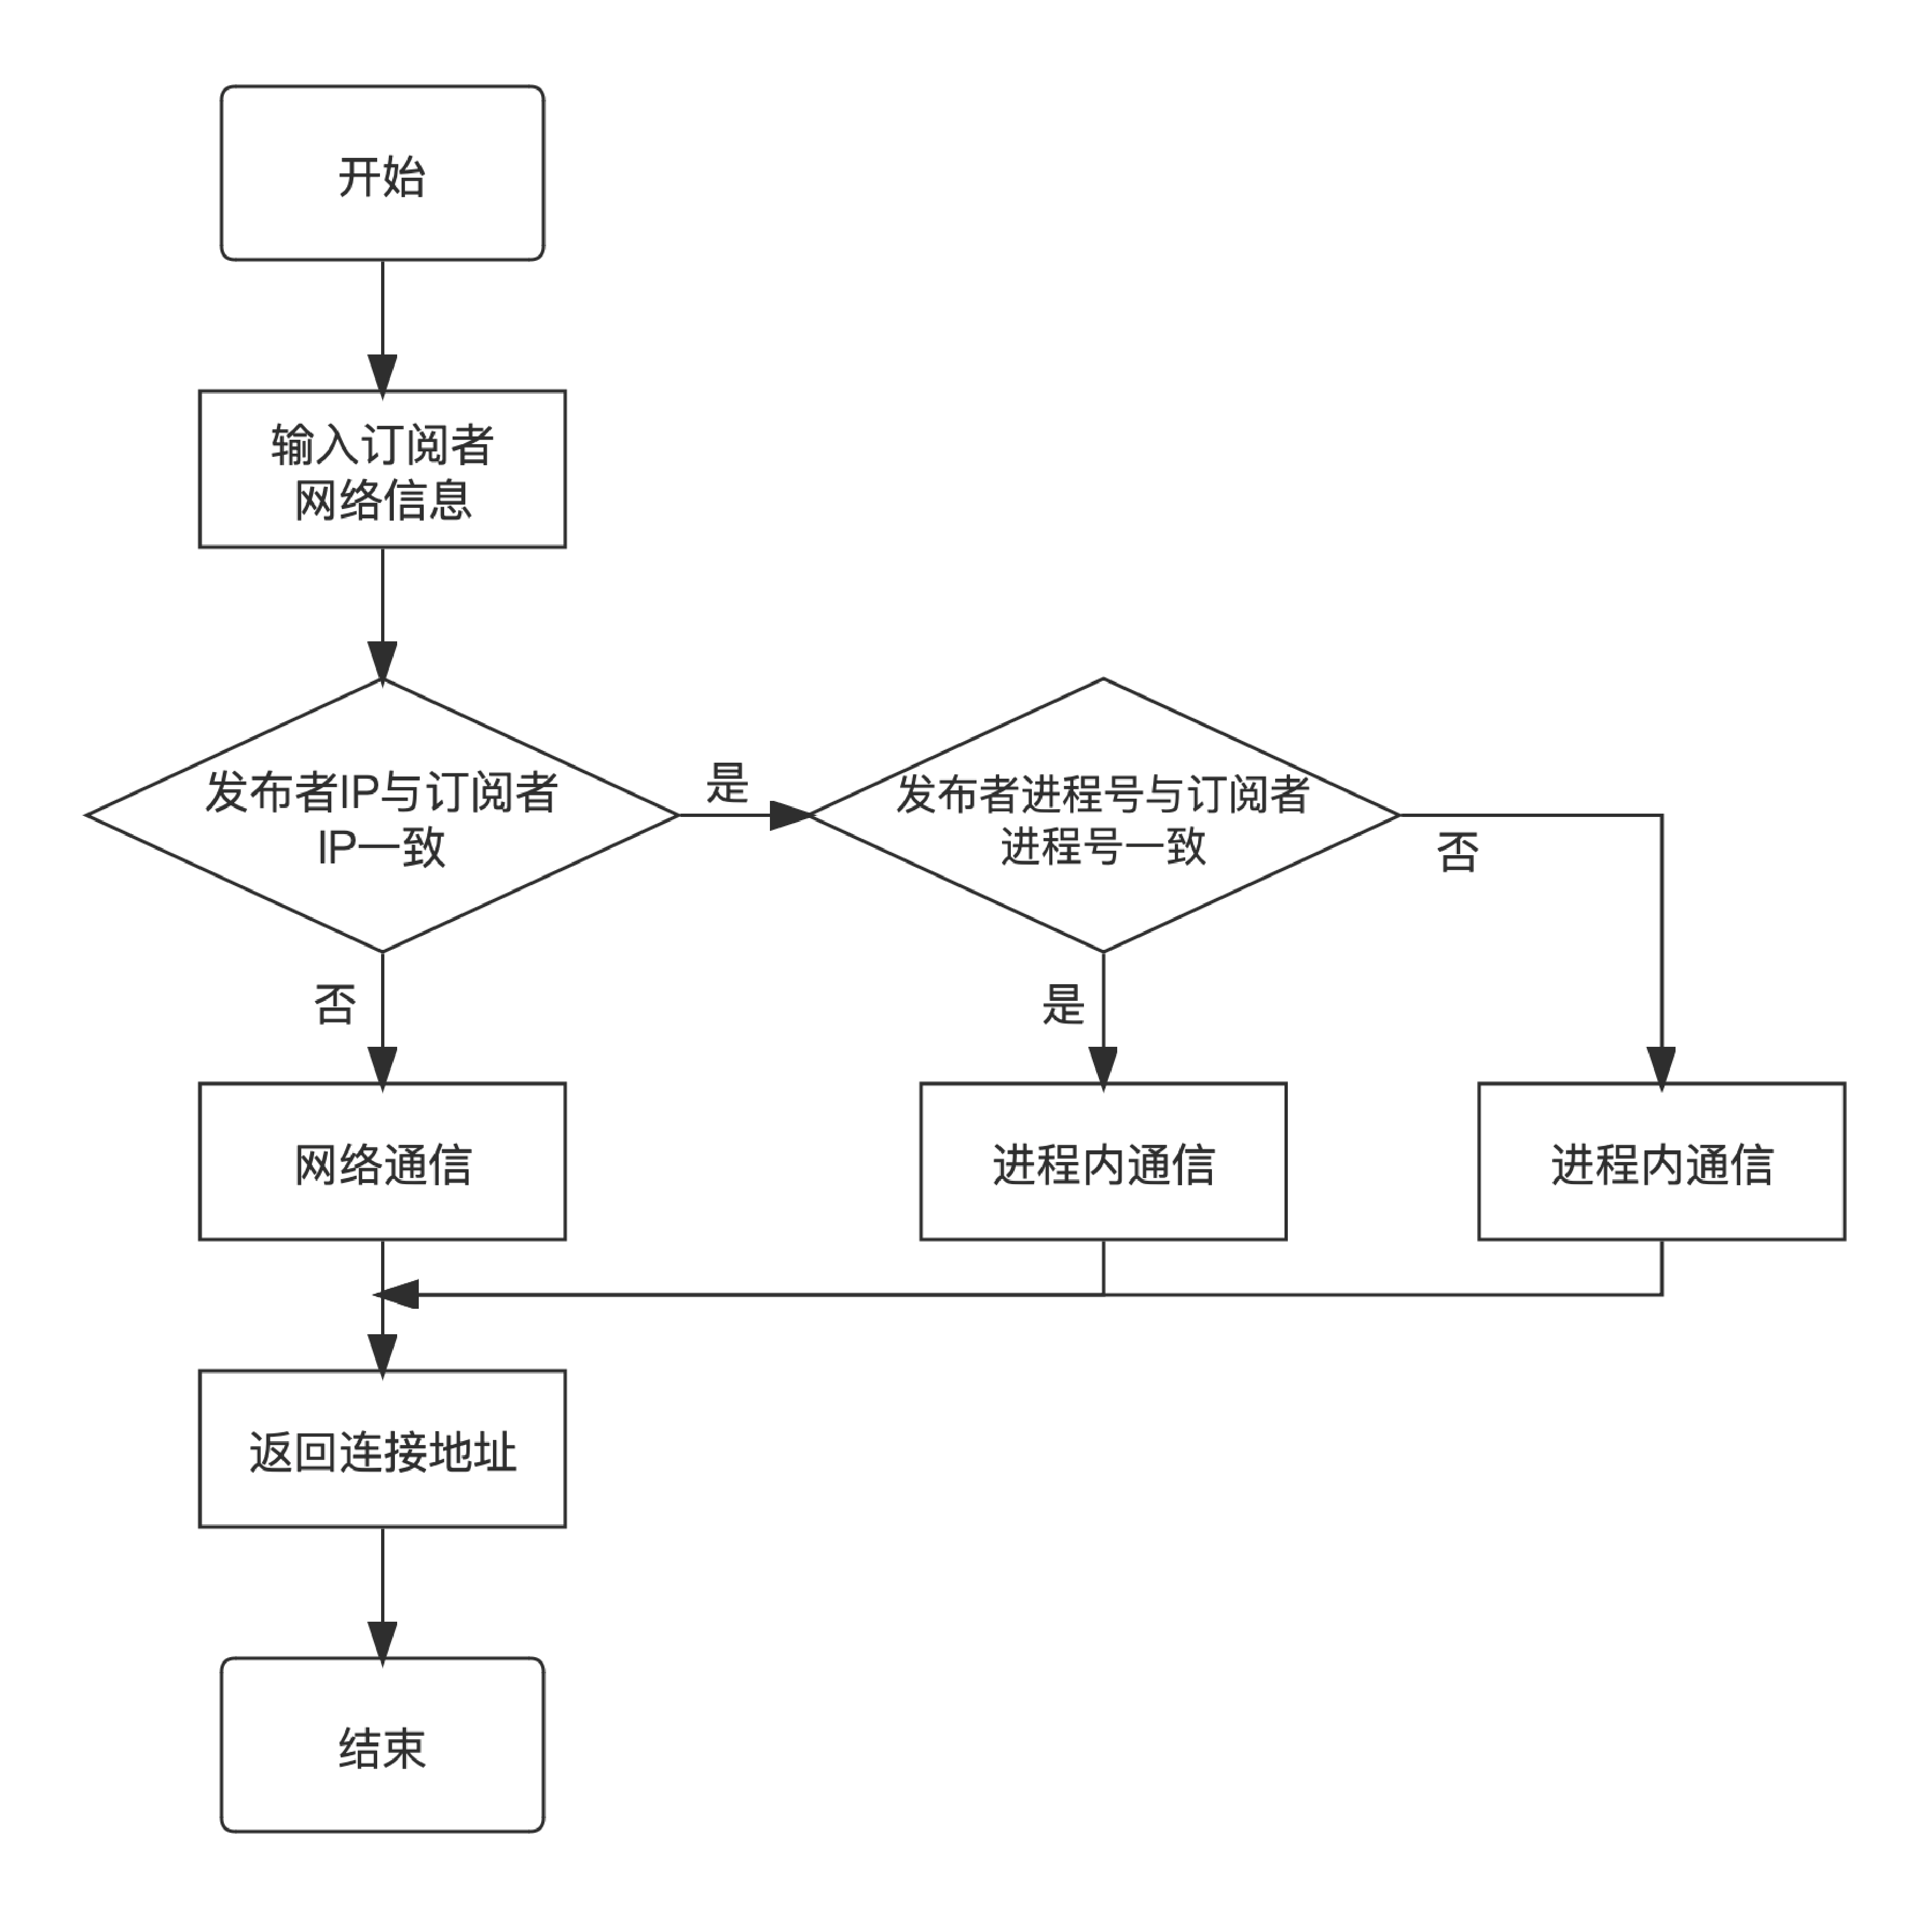
\includegraphics[width=0.65\textwidth]{adaptive_communication_select_flowchart.pdf}
  \caption{通信方式自适应选择流程图}
  \label{adaptive_communication_select_flowchart}
\end{figure}

\subsection{抽象订阅类概要设计}
抽象订阅类内部创建通信传输模块实现建立与发布者通信链路的建立以及消息的订阅,每个订阅者都唯一对应了一个抽象发布类
当有匹配的发布者时,服务发现模块将抽象发布类返回的连接地址作为参数传入订阅抽象类的回调函数中,回调函数中
通过对地址前缀的判断并连接至对应的通信链路,建立与发布者点对点的通信链路。通信方式自适应连接流程图如图\ref{adaptive_communication_connect_flowchart}所示。
\begin{figure}[H]
  \centering
  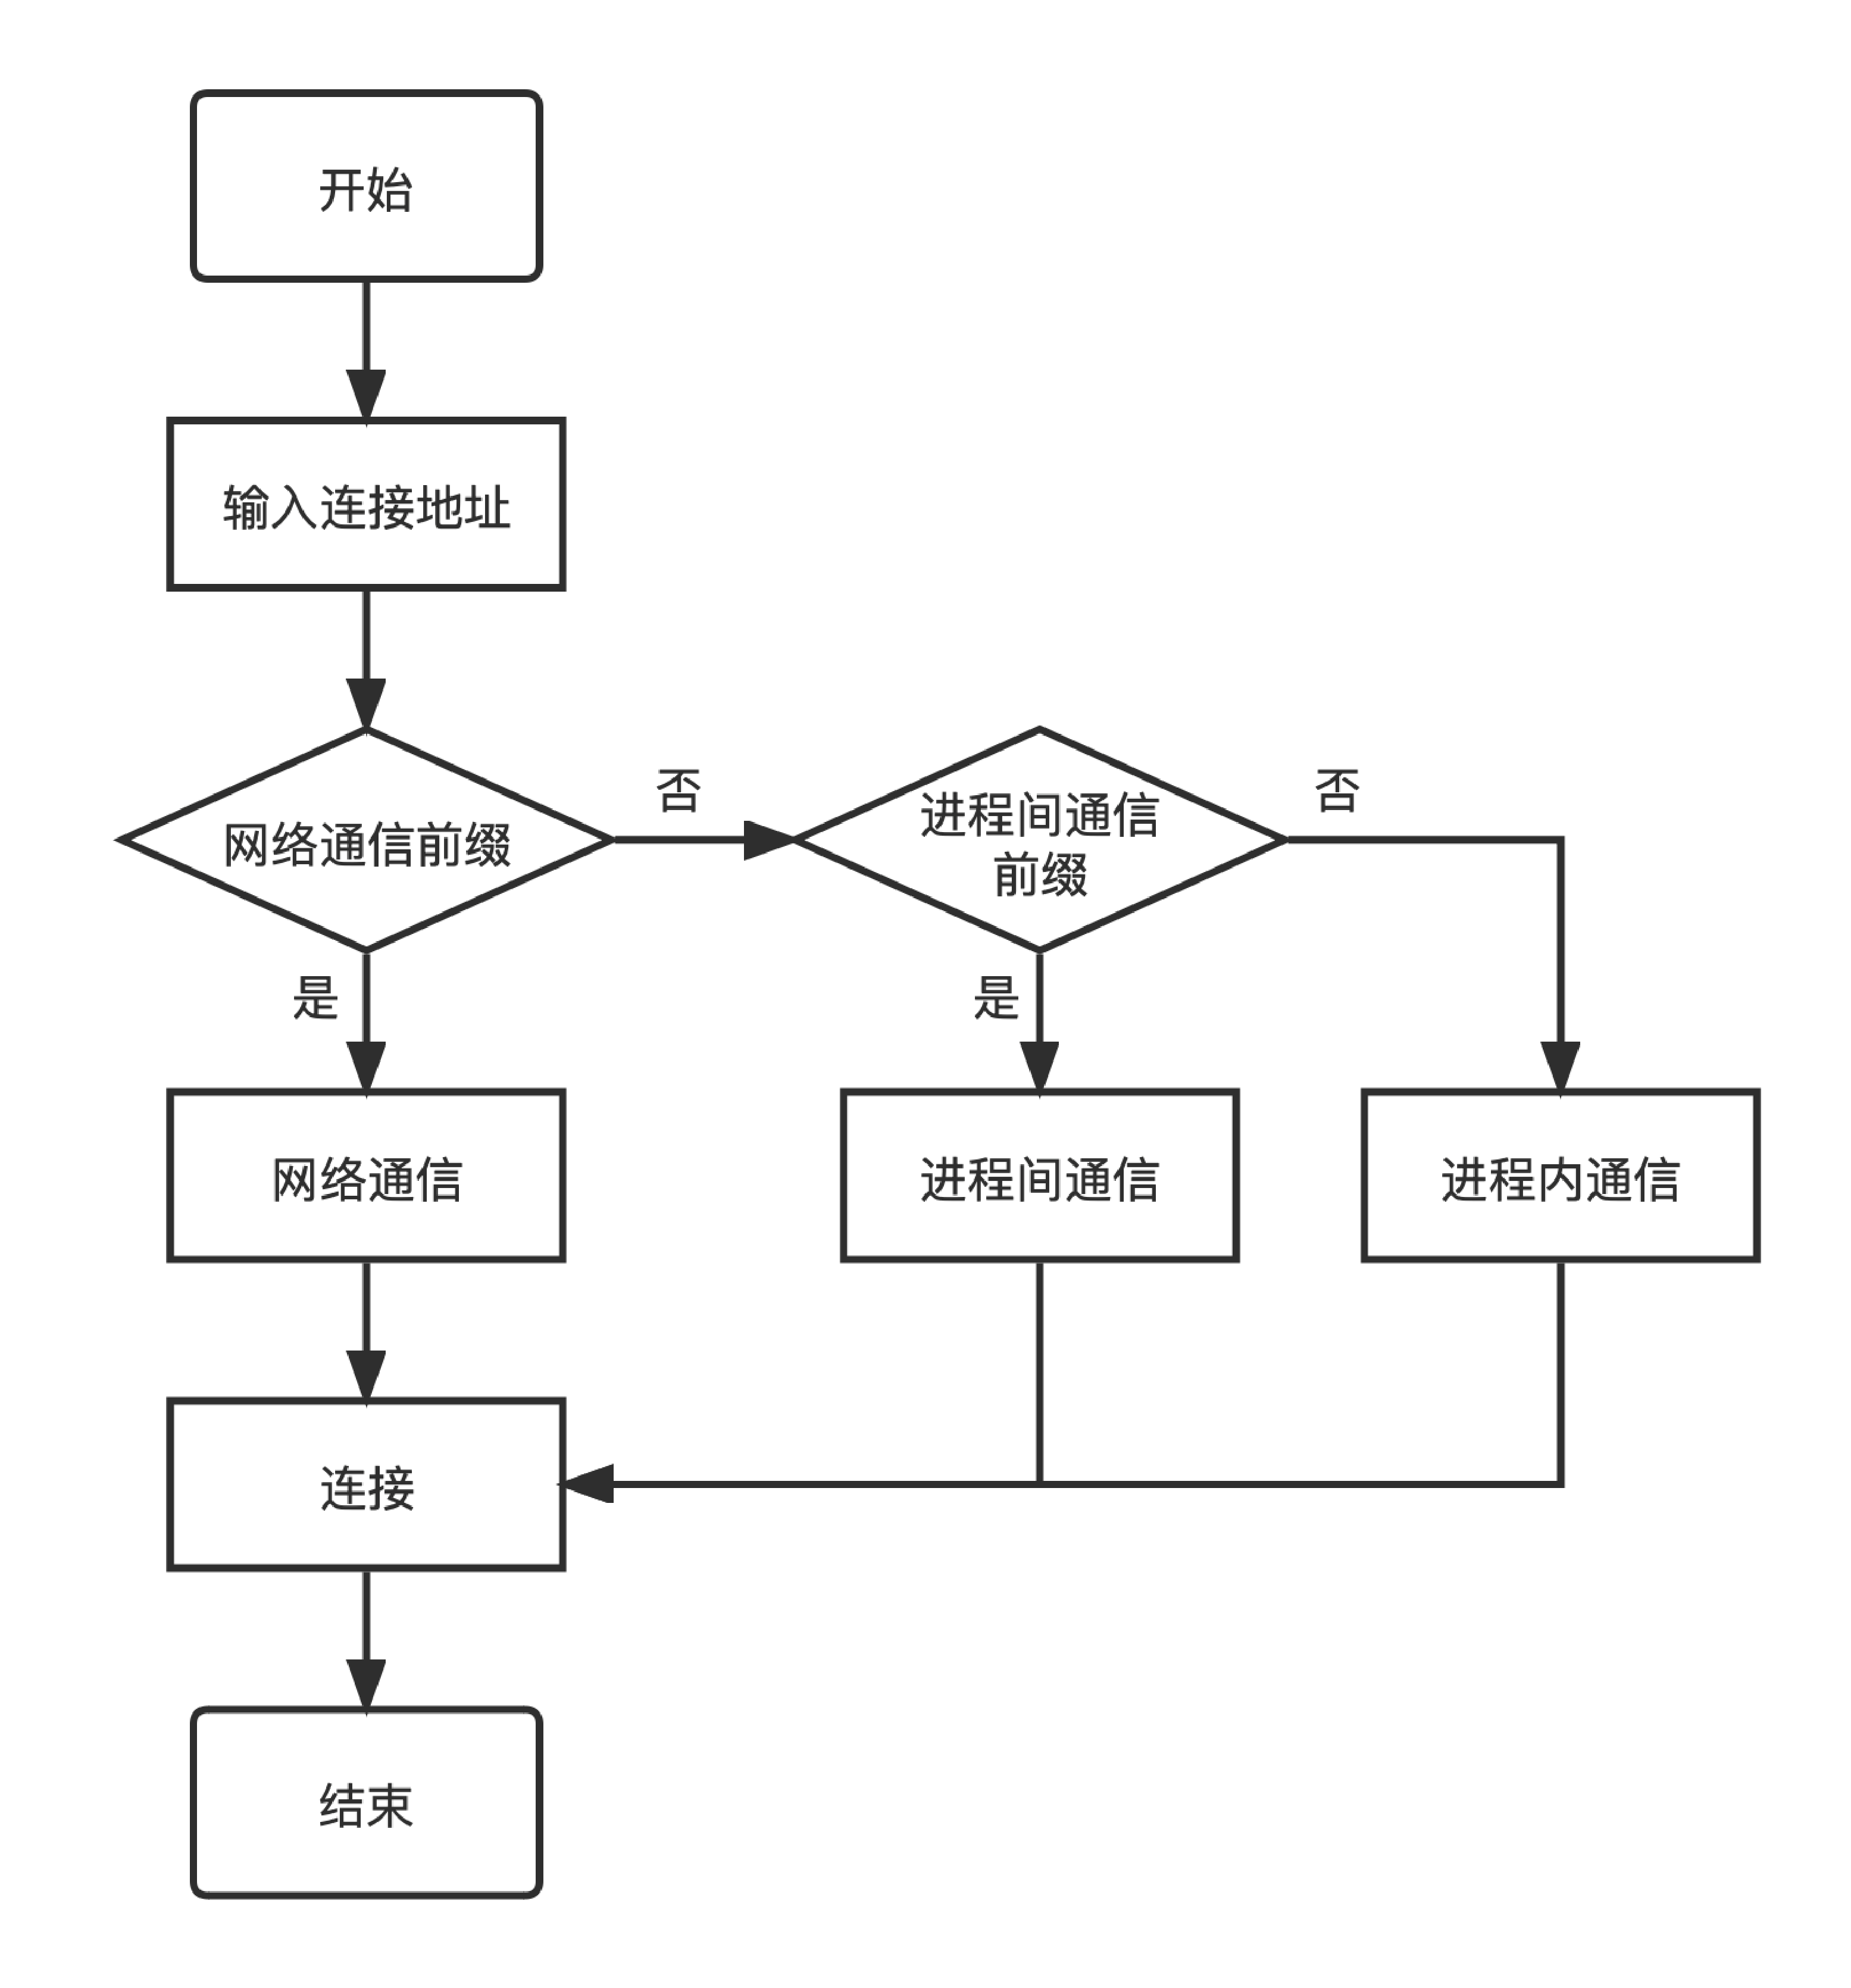
\includegraphics[width=0.65\textwidth]{adaptive_communication_connect_flowchart.pdf}
  \caption{通信方式自适应选择流程图}
  \label{adaptive_communication_connect_flowchart}
\end{figure}

\subsection{抽象服务类概要设计}
抽象服务类使用开源RPC框架rest\_rpc实现服务模块中服务端注册服务与客户端请求服务的功能,该类由通信抽象类
创建并唯一存在,即多个服务端和客户端共用一个抽象服务类。抽象服务类内部创建两个线程,一个线程用于接收客户端请求,
另一个线程用于发起服务请求和接收用户对客户端和服务的管理,两个线程处于异步运行状态。同一个进程中,抽象服务类
和服务发现模块的RPC服务共用一个端口。
抽象服务类时序设计如图\ref{abstract_service_gaiyao_shixu}所示。
\begin{figure}[H]
  \centering
  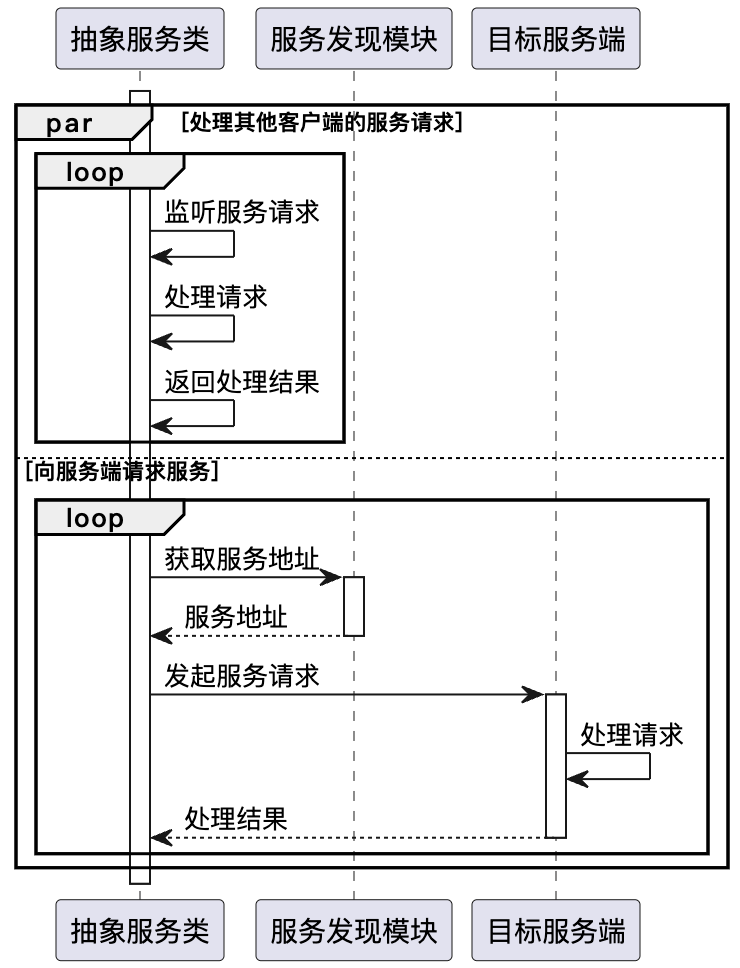
\includegraphics[width=0.45\textwidth]{abstract_service_gaiyao_shixu.png}
  \caption{抽象服务类时序设计}
  \label{abstract_service_gaiyao_shixu}
\end{figure}

\section{通信传输模块概要设计}
通信传输模块实现了本系统基于发布-订阅模式的通信功能,所有发布者与通信者的通信全部由本模块完成。
根据本系统提供的通信方式,通信传输模块分为进程间通信、进程内通信和网络通信三个子模块。

\subsection{进程内通信模块设计}
进程内通信模块的功能是实现同一个进程中的发布者与订阅者的通信。进程内通信模块的创建与删除由抽象发布类和抽象
订阅类管理,二者共用一个进程内通信模块实例。抽象发布类通过该模块管理进程内发布者,抽象订阅类通过该模块管理
进程内订阅者。

进程内通信模块包含一个进程内通信管理类、一个进程内通信发布者类和一个进程内通信订阅者类。进程内通信管理类负责创建、删除
进程内通信下的发布者与订阅者,并开辟线程轮询消息队列是否有新消息的到来;进程内通信发布者类负责将待发布消息压入消息队列中;
进程内订阅者类负责从消息队列弹出订阅消息,并调用用户传入的回调函数将消息压入订阅者模块中的消息队列中供用户使用。

由于发布者与订阅者处于同一个进程内,二者间的通信
不需要使用网络通信或共享内存,只需要传递消息的指针即可完成通信,不需要对消息进行额外拷贝。进程内通信模式下,
使用同一个话题通信的发布者与订阅者共用一个消息队列,发布者将消息的指针存入消息队列,而订阅者将消息的指针从
消息队列中取出,进程内通信模块消息传输设计如图\ref{intraprocess_gaiyao}所示。从图\ref{intraprocess_gaiyao}可以看出,进程内通信模块根据话题创建不同的消息
队列,使用同一个话题通信的发布者与订阅者通过向消息队列压入或弹出消息的方式进行通信。同时,本模块为了保证消息
队列在发布者执行压入消息和订阅者执行弹出消息操作时的原子性,使用了互斥锁机制对临界资源即消息队列进行保护。
\begin{figure}[H]
  \centering
  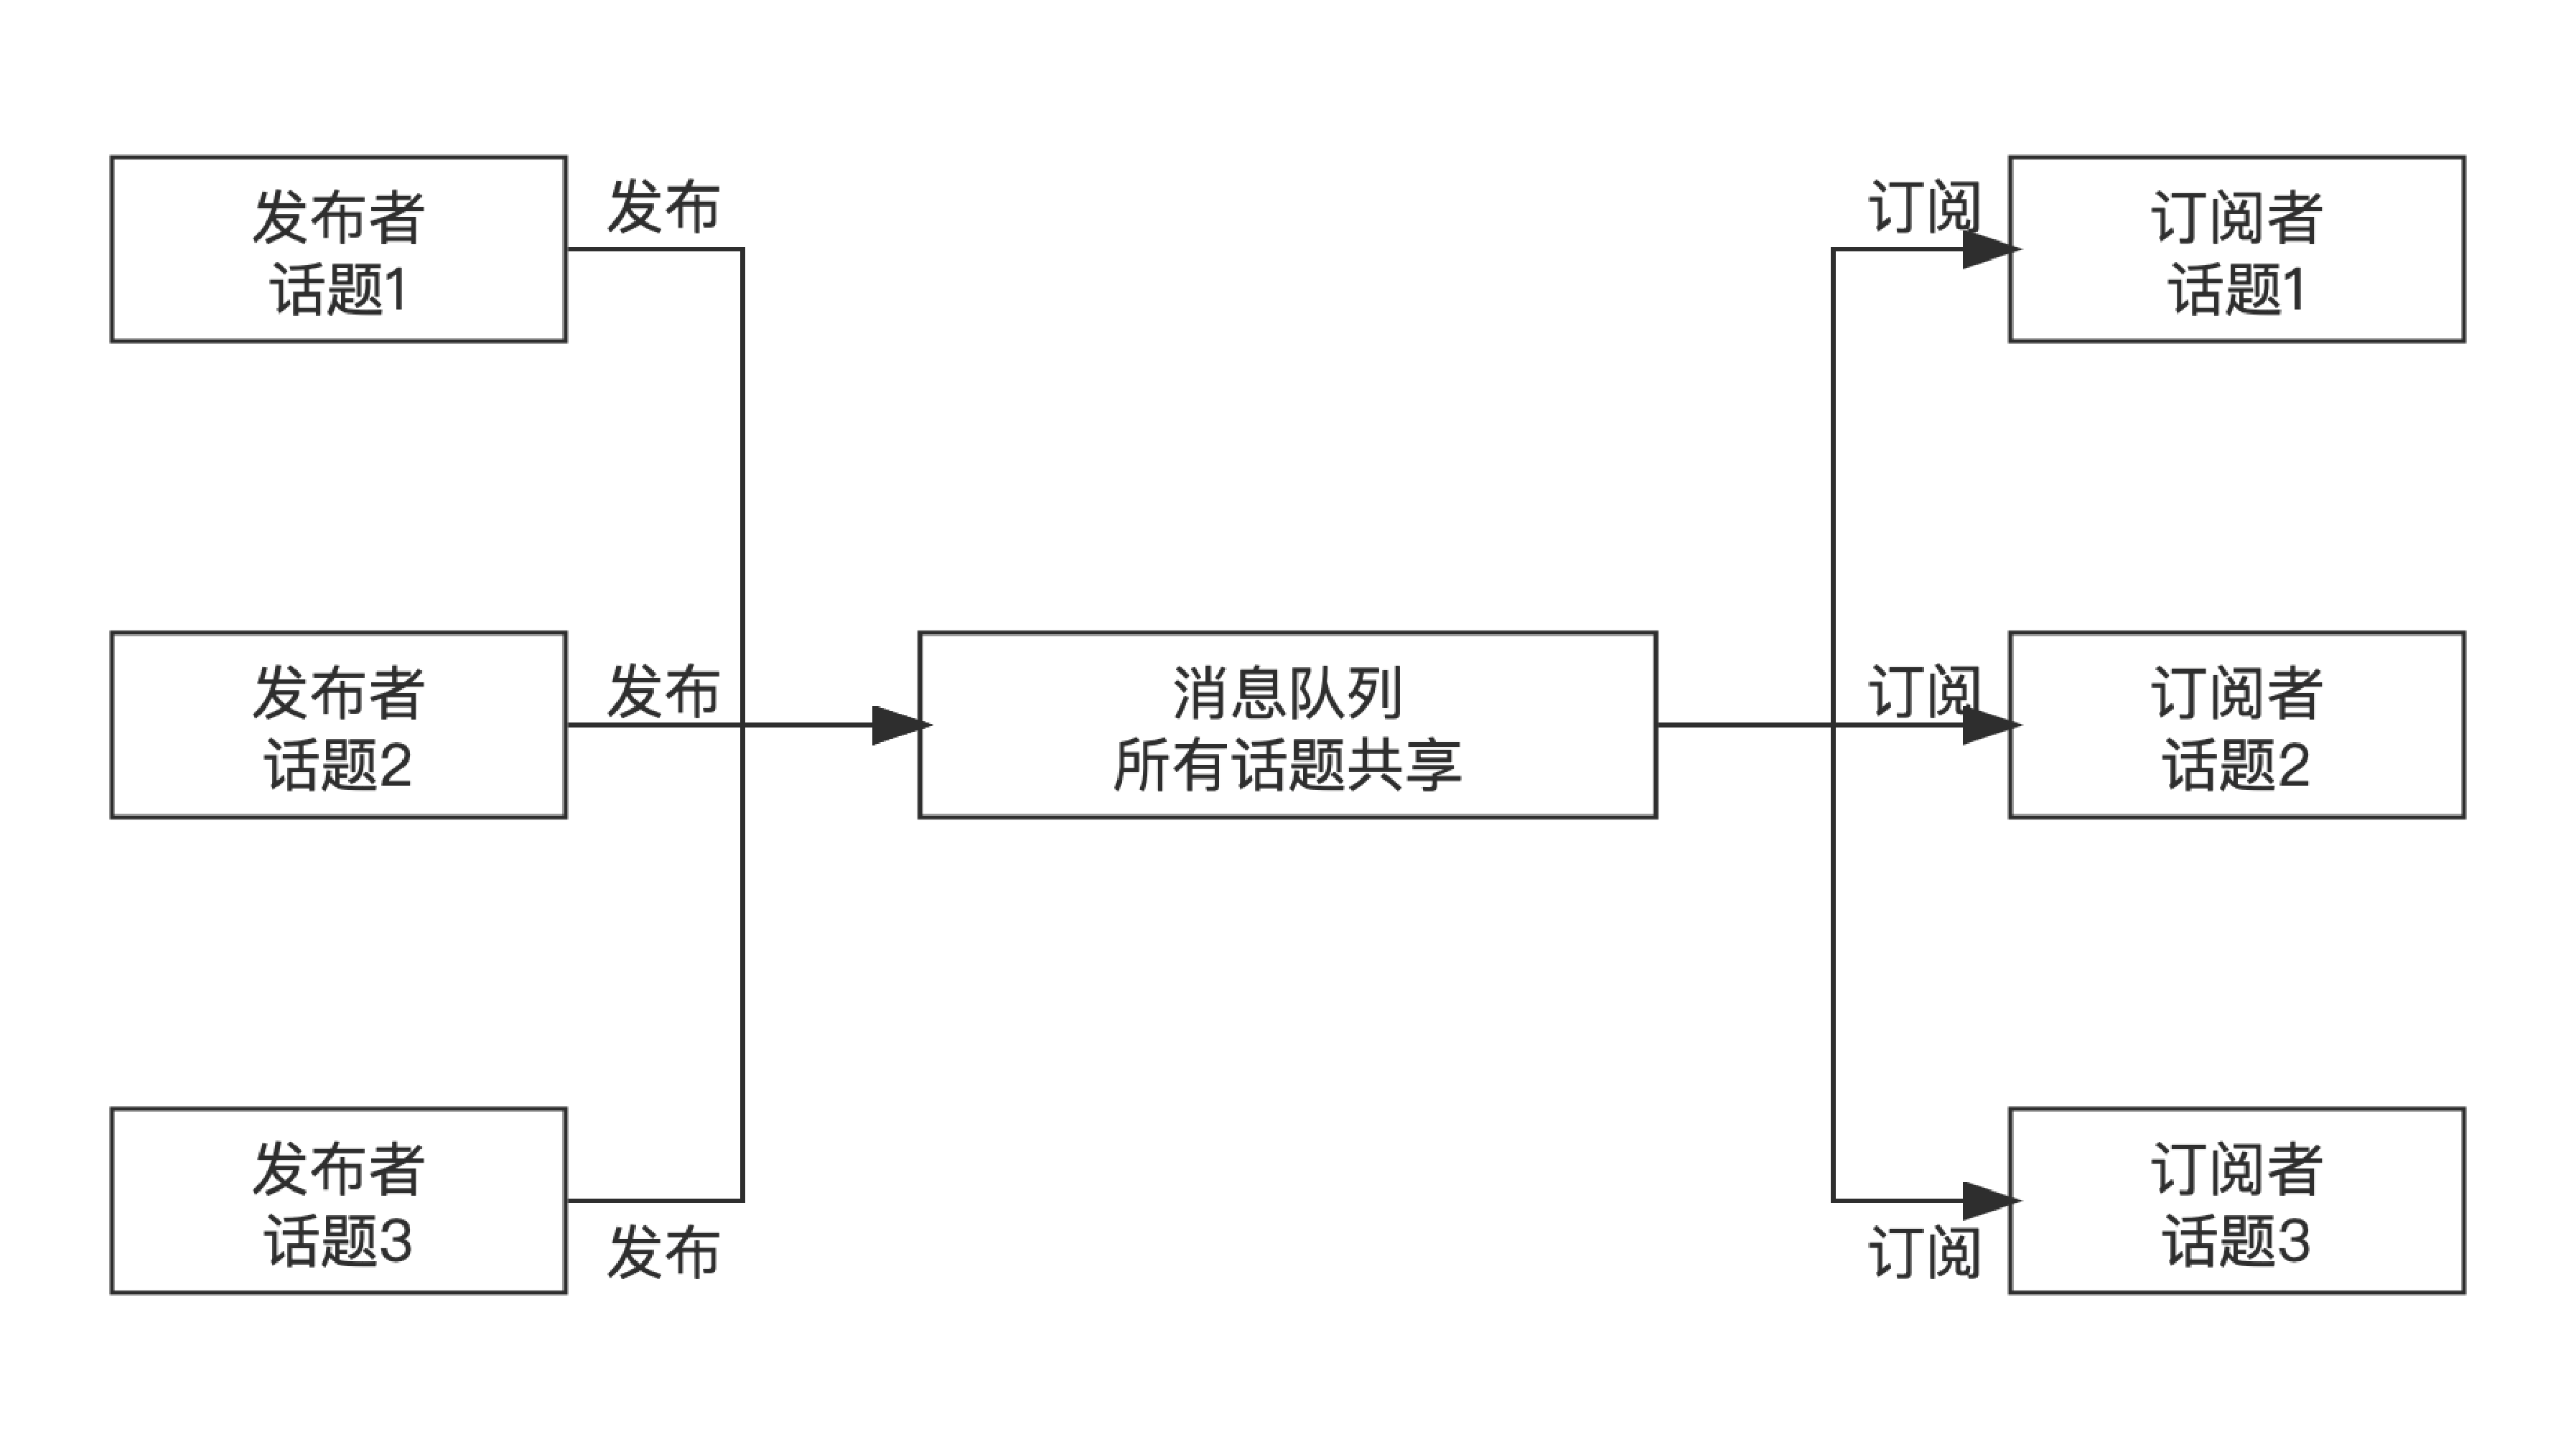
\includegraphics[width=0.9\textwidth]{intraprocess_gaiyao.pdf}
  \caption{进程内通信消息传输}
  \label{intraprocess_gaiyao}
\end{figure}

\subsection{进程间通信模块概要设计}
进程间通信模块的功能是使用共享内存实现同一台物理机不同进程中的发布者与订阅者的通信。进程间通信模块的创建与删除
由抽象发布类和抽象订阅类管理,二者共用一个网络通信模块实例。

进程间通信模块包含一个进程间通信管理类、一个进程间通信发布者类和一个进程间通信订阅者类。进程间通信管理类负责创建、
删除进程间通信下的发布者类与订阅者类,并开辟线程轮询是否有新的消息到来;进程间通信发布者类负责将待发布消息
进行序列化处理,然后将序列化后的消息写入对应共享内存文件,通过ZeroMQ PUB套接字通知对应订阅者接收消息;进程间通信订阅者类
通过ZeroMQ SUB套接字接收发布者的通知并从共享内存文件中取出对应的消息并进行反序列化操作,最后调用用户传入的回调函数
将消息压入订阅者模块中的消息队列中供用户使用。进程间通信模块传输设计如图\ref{interprocess_gaiyao}所示。
\begin{figure}[H]
  \centering
  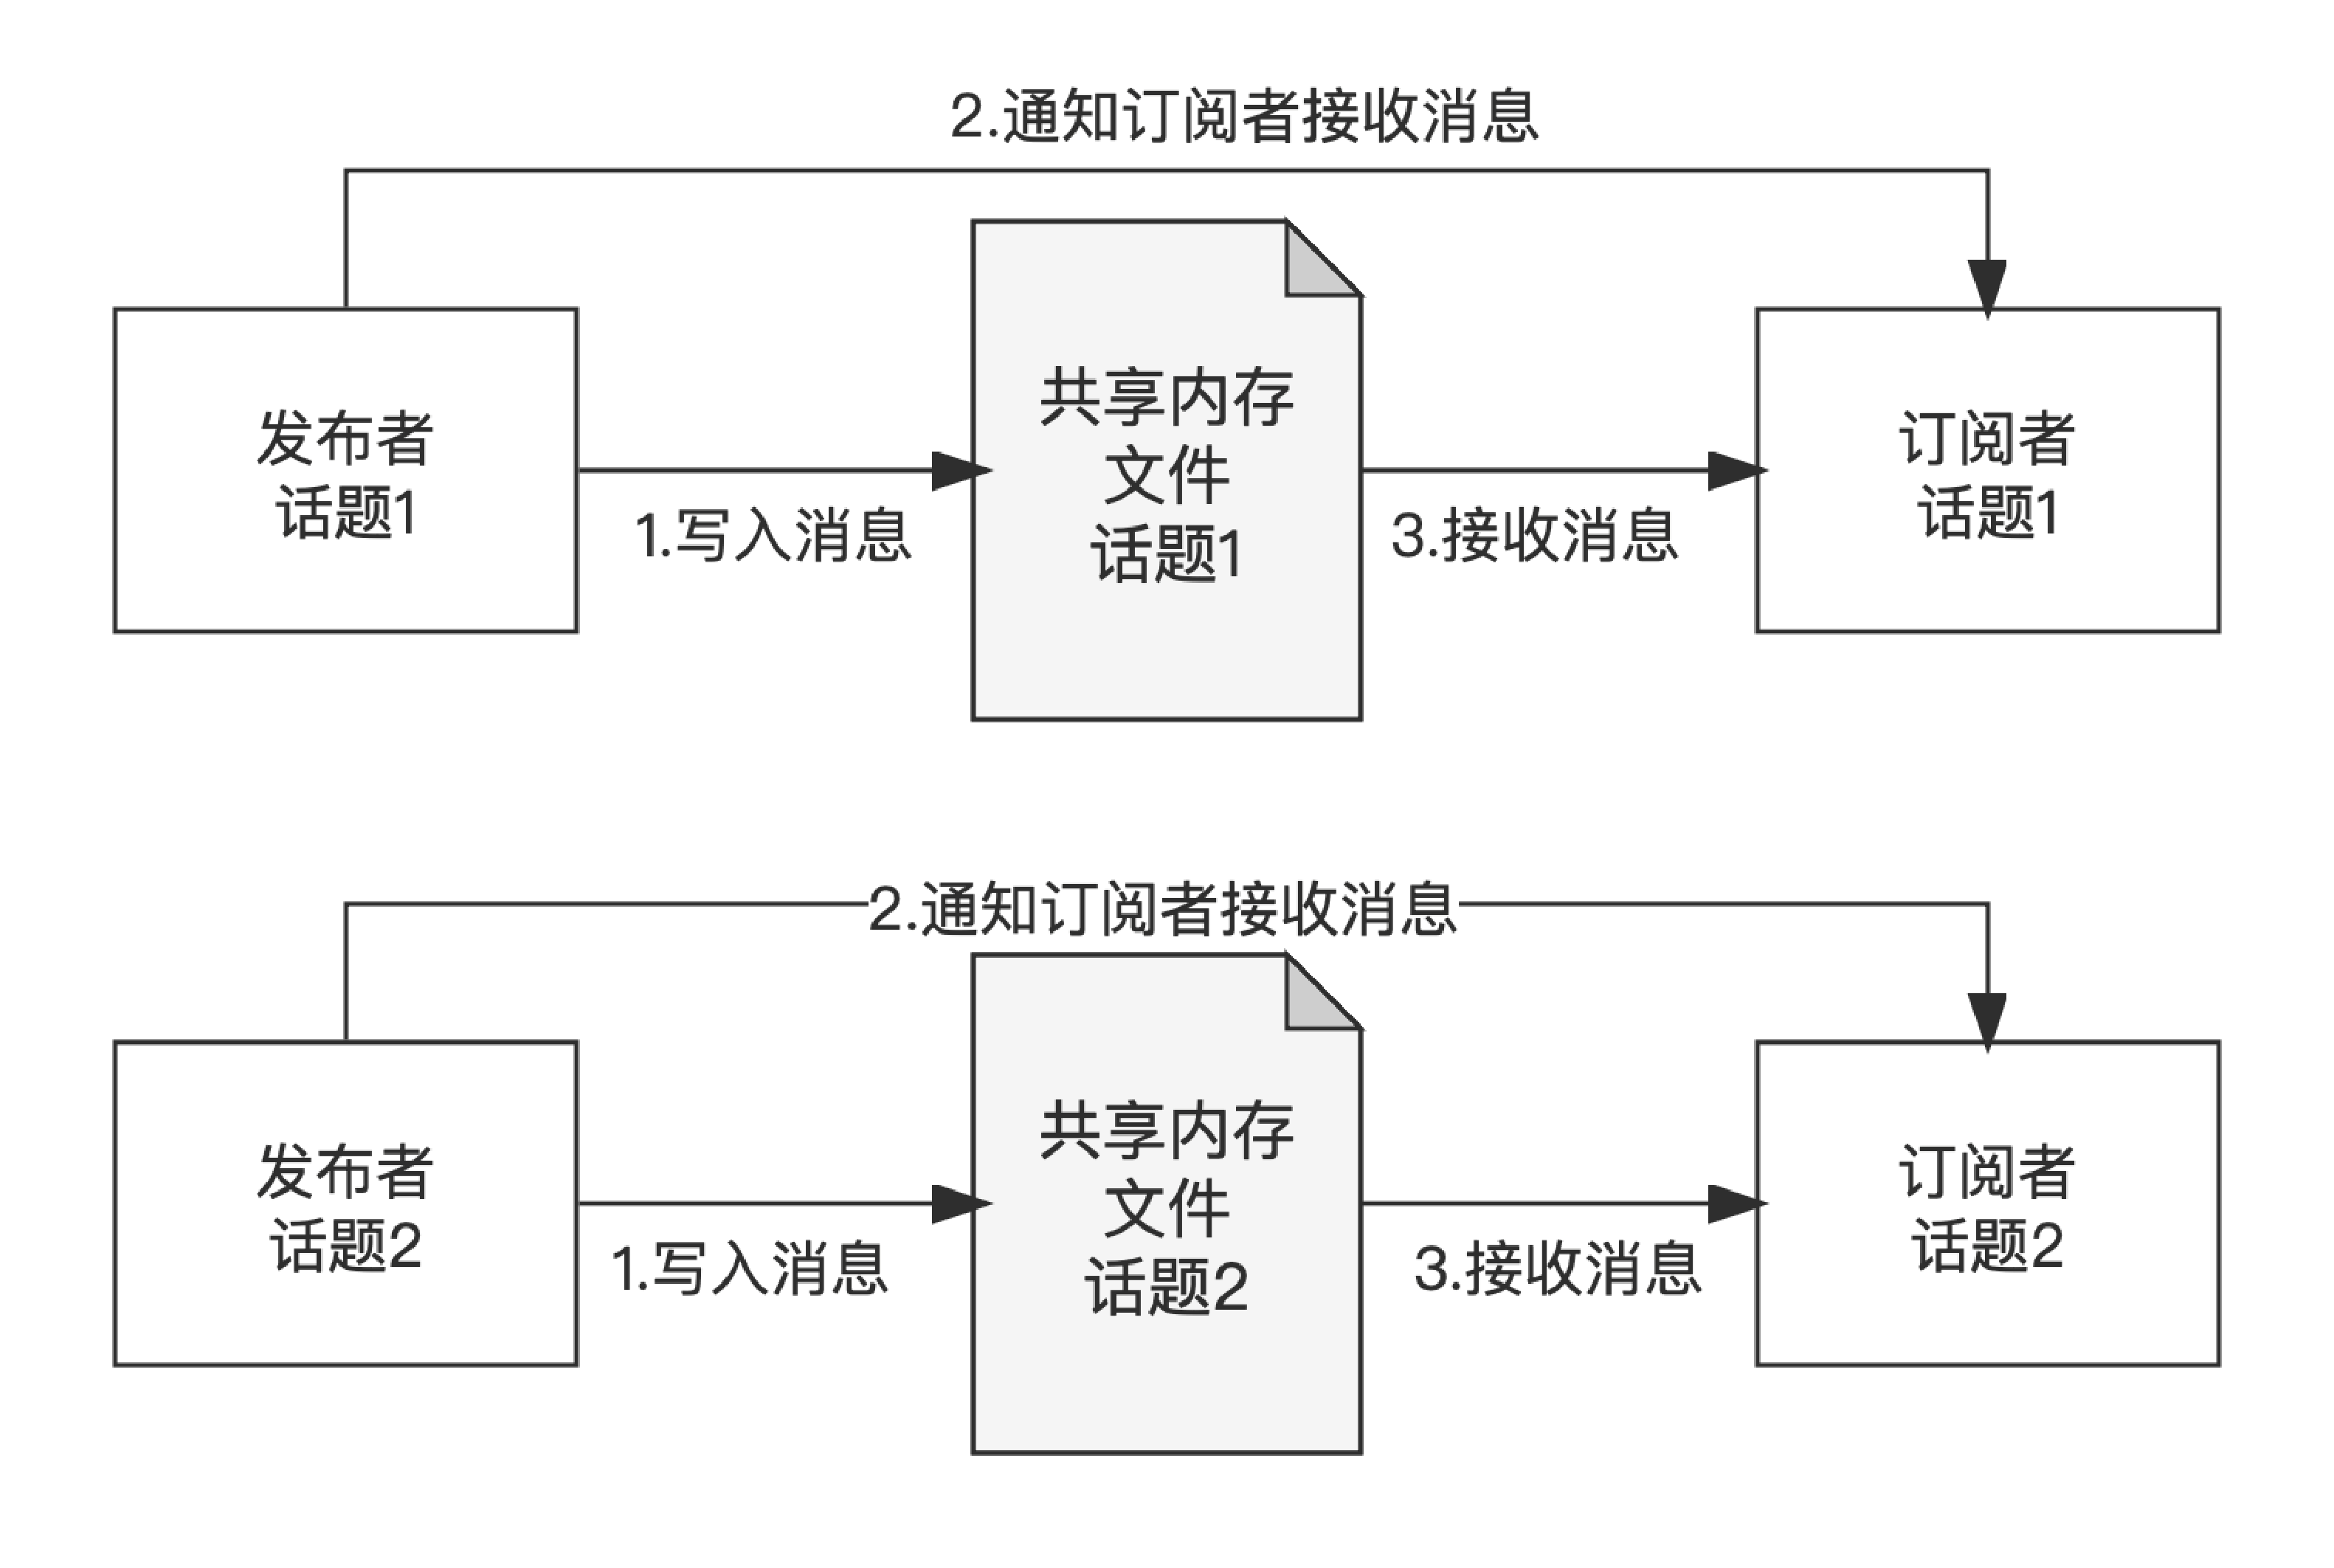
\includegraphics[width=0.8\textwidth]{interprocess_gaiyao.pdf}
  \caption{进程间通信消息传输}
  \label{interprocess_gaiyao}
\end{figure}

\subsection{网络通信模块概要设计}
网络通信模块的功能是使用ZeroMQ实现不同物理机建间的发布者与订阅者的通信。网络通信模块的创建与删除由抽象发布类和抽象订阅类
管理,二者共用一个网络通信模块实例。

\begin{figure}[H]
  \centering
  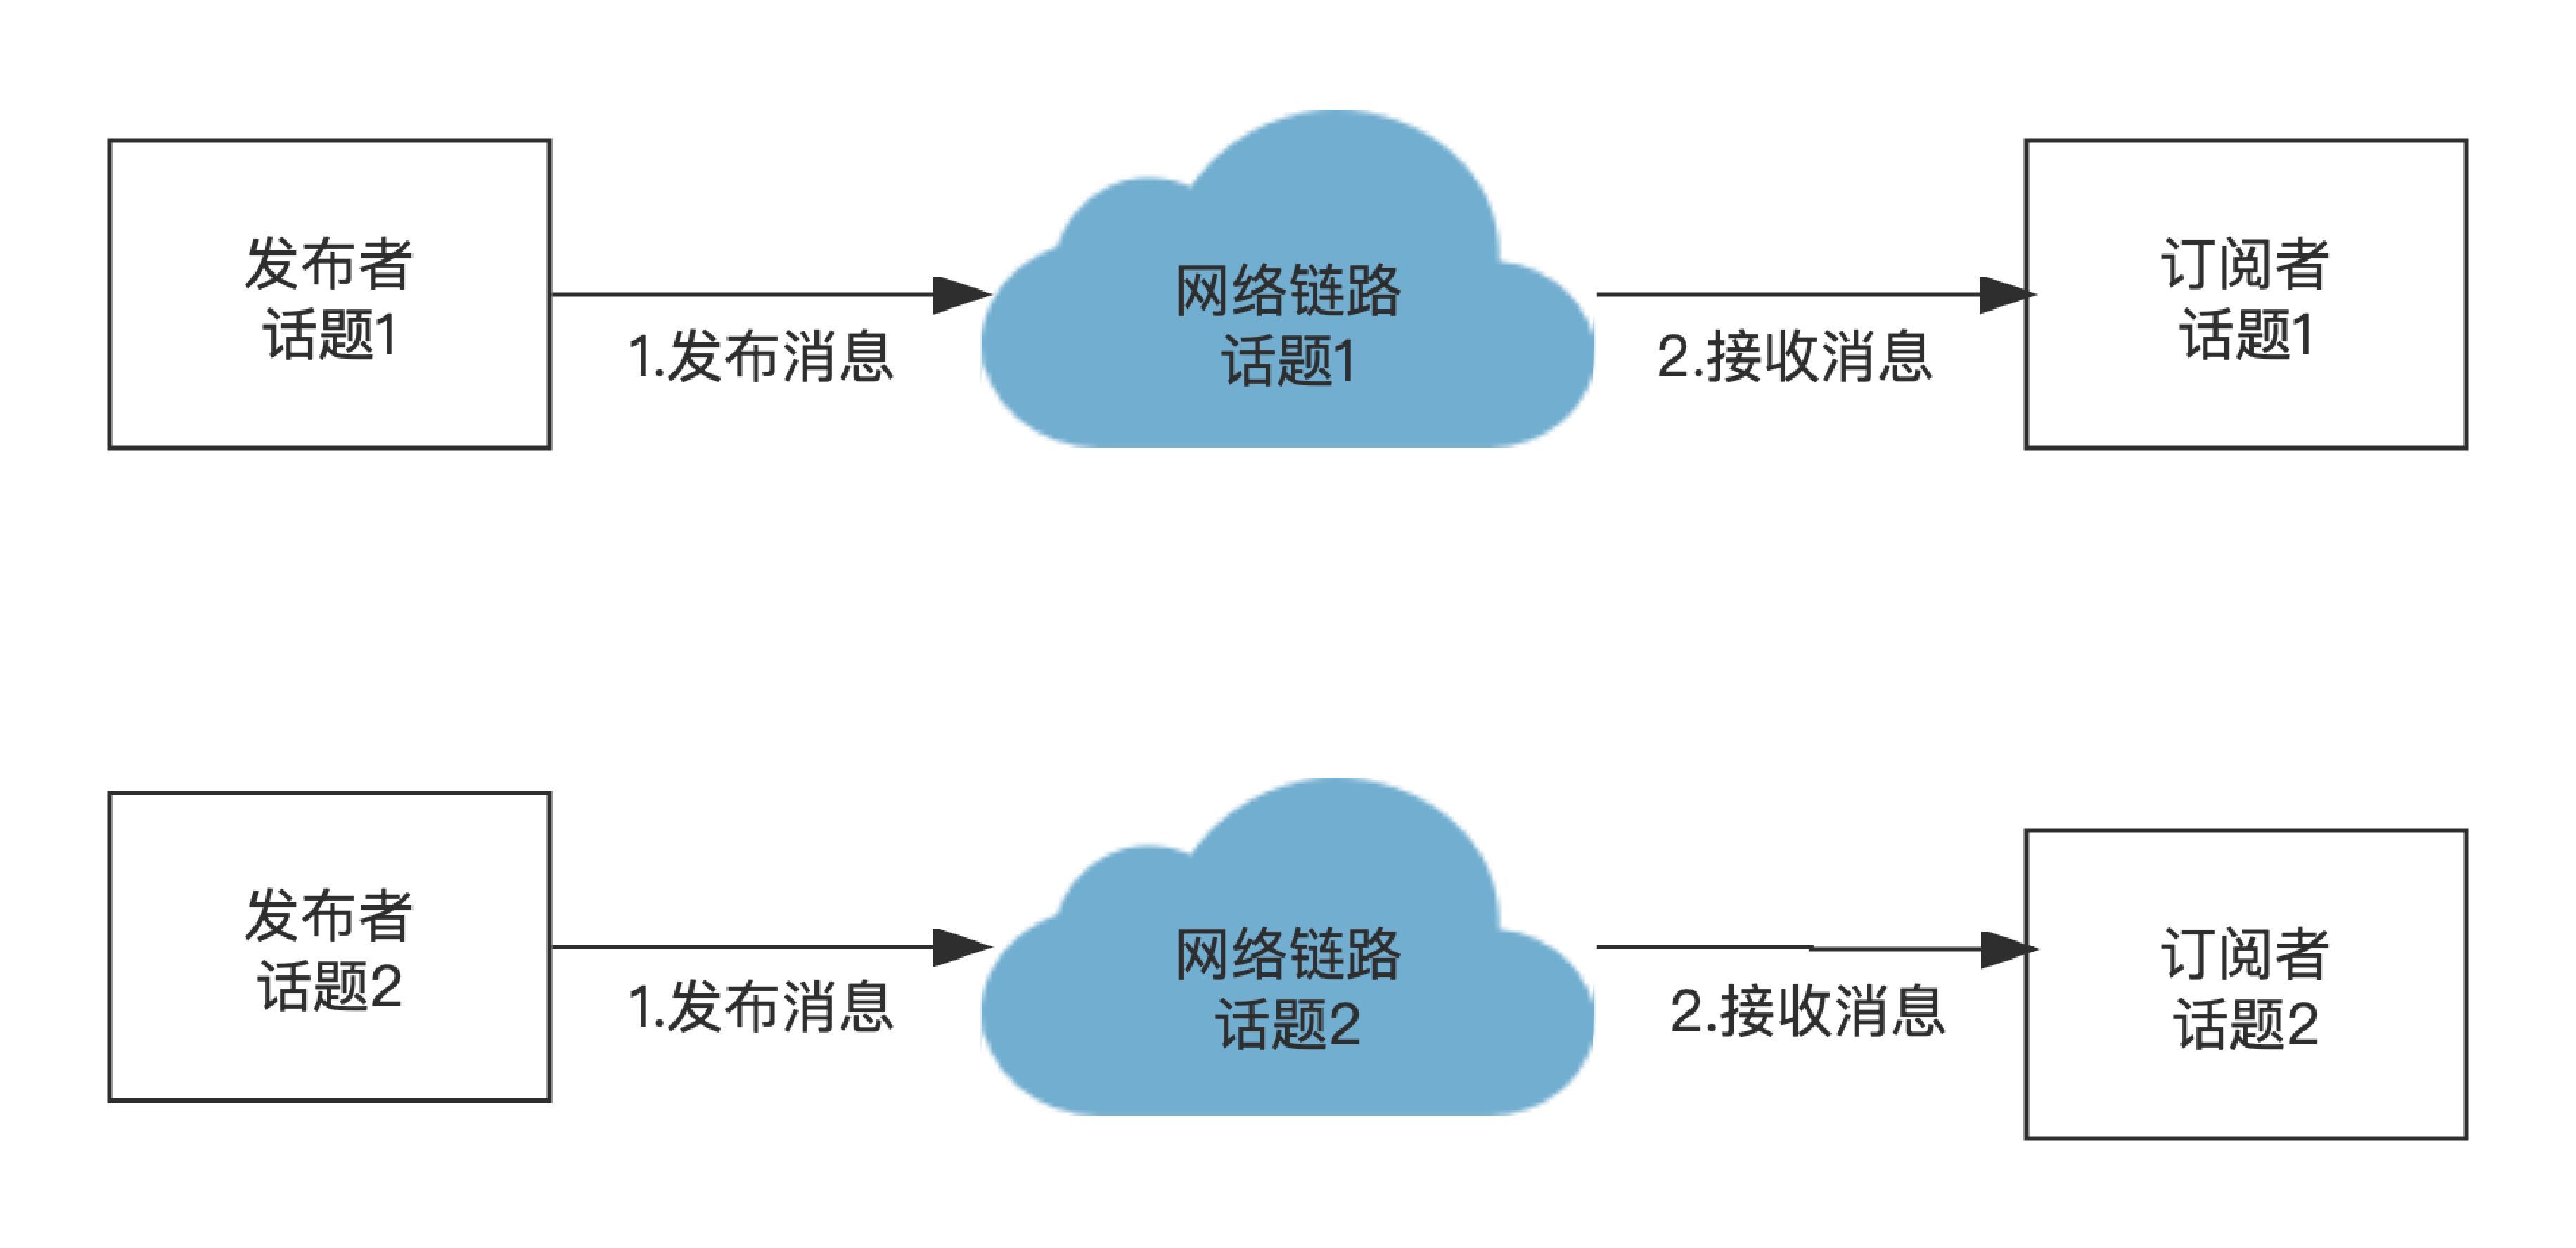
\includegraphics[width=0.8\textwidth]{network_gaiyao.pdf}
  \caption{网络通信消息传输}
  \label{network_gaiyao}
\end{figure}

网络通信模块消息传输设计如图\ref{network_gaiyao}所示。
网络通信模块基于ZeroMQ中的PUB-SUB套接字完成,传输协议使用ZeroMQTCP协议。
网络通信模块包含一个网络通信管理类、一个网络通信发布者类和一个网络通信订阅者类。网络通信管理类负责创建、删除网络通信
下的发布者与订阅者,并开辟线程轮询网络链路是否有新的消息到来;网络通信发布者类负责将待发布消息进行序列化处理,然后
通过ZeroMQ PUB套接字发送;网络通信订阅者类通过ZeroMQ SUB套接字从网络链路中取出消息并对消息进行反序列化,最后调用用户传入的回调函数将
消息压入订阅者模块中的消息队列中供用户使用。

\subsection{消息模块概要设计}
消息模块向网络通信模块和进程间通信模块提供消息的序列化和反序列化功能。
本系统使用protobuf作为消息的序列化与反序列化的工具。protobuf需要由用户根据业务需要的数据结构
编写后缀名为.proto的IDL文件并使用protobuf提供的protoc工具生成与.proto文件对应的.pb.h文件和.pb.cc文件,
用户通过引用.pb.h文件中的C++接口实现对消息的序列化与反序列化,但.pb.h中的接口与C++原生数据结构(int,vector等)
在赋值等场景下的使用方法并不相同,本系统基于protobuf生成的.pb.h与.pb.cc文件二次生成一套C++代码。
\begin{figure}[H]
  \centering
  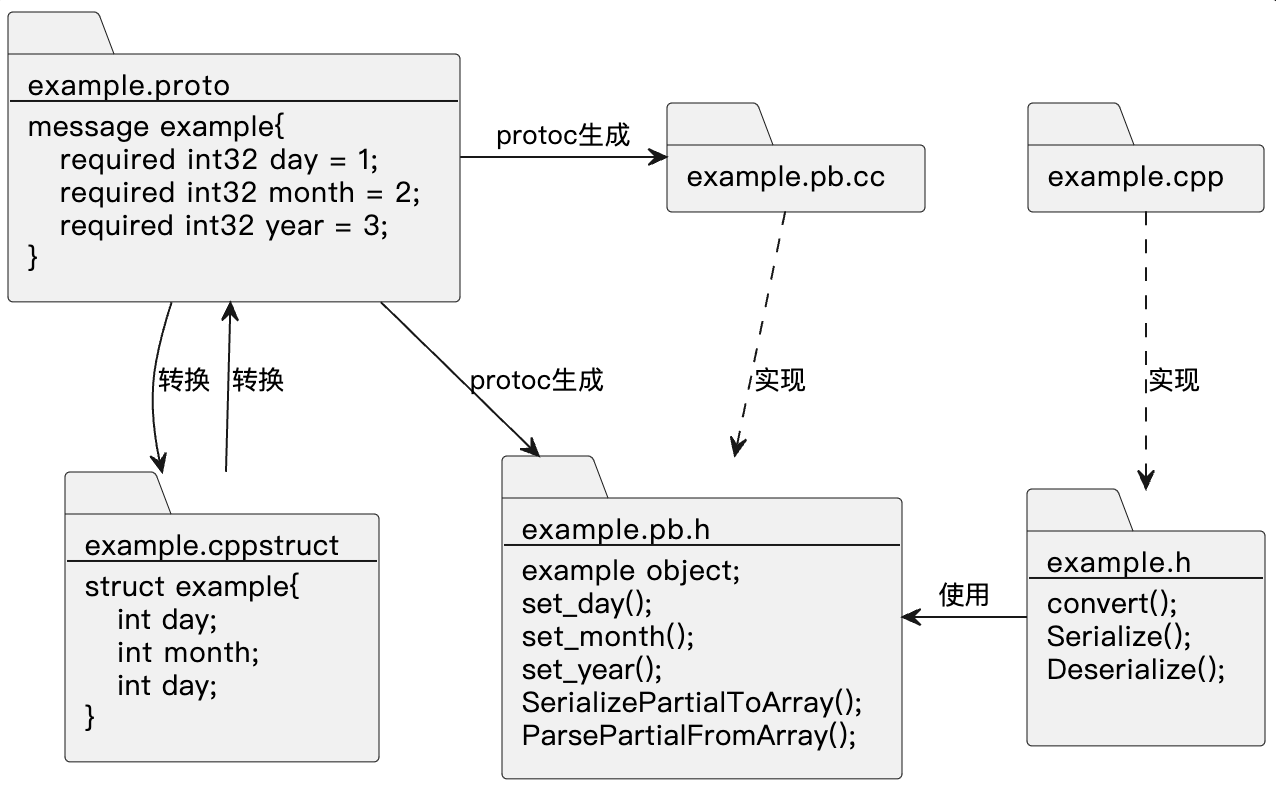
\includegraphics[width=0.8\textwidth]{message_proto_struct_convert.png}
  \caption{中间语言代码文件关系}
  \label{proto-struct-convert}
\end{figure}

如图\ref{proto-struct-convert}所示,中间语言的代码向用户提供与.proto文件对应的原生C++数据结构,用户在发布者类和订阅者类中使用原生C++数据结构进行对消息的处理。但在
网络通信模块和进程间通信模块发布消息时,中间语言通过protobuf接口将原生的C++数据结构转换为protobuf接口并调用
protobuf提供的序列化接口将转换后的结构序列化后发布消息;在网络通信模块和进程间通信模块接收消息时,中间语言通过protobuf提供的
反序列化接口先将消息反序列化为protobuf结构,再将protobuf结构转换为原生C++结构。



\section{服务发现模块概要设计}
服务发现模块是实现本系统实现动态网络下通信功能的重要模块,服务发现模块唯一存在于每个进程。

服务发现模块根据抽象服务类以及中心发出的服务发现请求参数实现服务发现功能,服务发现请求参数如表\ref{service_discovery_parameter}所示。
服务发现模块服务发现机制分为两类:主动发现和被动发现。
一方面,通信抽象类在本机内新增、删除或修改发布者、订阅者以及服务服务端时导致网络拓扑变化时向服务发现模块发出请求,服务发现模块主动向中心节点发出发现请求获取匹配通信方信息;
另一方面,在其他进程中中网络拓扑发生变化时其自身的服务发现模块会向中心节点发出发现请求获取匹配通信方信息,中心节点会自动寻找
相关联的服务发现模块并发出更新信息查询请求,关联的服务发现模块根据更信息更新通信链路。服务发现模块的服务发现功能的工作流如下:
\begin{enumerate}
  \item 本进程内新增、删除或修改发布者,服务发现模块将通信抽象类发出的请求参数通过RPC更新该发布者信息至中心节点,并将参数保存至本模块。
  中心节点按服务发现模块查询匹配的订阅者信息,若查询到则将所有关联的其他进程中的服务发现模块的RPC地址和订阅者信息返回至本进程服务发现模块。
  本进程服务发现模块将每个订阅者网络信息作为参数调用抽象发布类的更新通信链路回调函数完成自适应通信方式连接后,通过RPC将连接地址和订阅者信息
  发送给每一个其他进程的服务发现模块。其他进程的服务发现模块根据连接地址调用抽象订阅类中的更新通信链路回调函数完成自适应通信连接。
  匹配的发布者与订阅者连接至同一个连接地址,双方开始通信。
  \item 本进程内新增、删除或修改订阅者,服务发现模块将通信抽象类发出的请求参数通过RPC更新该订阅者信息至中心节点,并将参数保存至本模块。
  中心节点按服务发现模块查询匹配的发布者信息,若查询到则将本进程服务发现模块的RPC地址和订阅者网络信息通过RPC发送至所有关联的其他进程中的
  服务发现模块。其他进程的服务发现模块根据订阅者网络信息完成自适应通信方式连接后将连接地址和订阅者网络信息通过RPC发送至本进程的服务发现模块。本进程服务发现模块
  根据连接地址完成自适应通信连接,双方开始通信。
  \item 本进程内新增、删除或修改服务服务端,服务发现模块将通信抽象类发出的请求参数通过RPC更新该服务服务端信息至中心节点,并将参数保存至本模块。
  更新完成后,不需要与关联的客户端建立通信链路。其他进程的客户端仅在向请求本进程中的服务时通过其服务发现模块向中心节点请求
  服务所在IP地址。
  \item 本机进程内新增、删除或修改服务客户端,服务发现模块仅保存参数,并不向中心节点发起RPC请求。
  \item 其他进程内新增、删除或修改发布者,其他进程的服务发现模块会将订阅者网络信息和连接地址通过RPC的方式通知本进程的服务发现模块。
  本进程服务发现模块根据订阅者信息查询到与其对应的抽象订阅类,将连接地址作为参数调用抽象订阅类的更新通信链路回调函数完成自适应通信方式连接,
  双方开始通信。
  \item 其他进程内新增、删除或修改订阅者,
  中心节点会将其他进程的服务发现模块的RPC地址和订阅者网络信息通过RPC通知本进程的服务发现模块。本进程服务发现模块根据订阅者网络信息
  查询到对应的抽象发布类,将订阅者网络信息作为参数调用抽象发布类的更新通信链路回调函数完成自适应通信方式连接,最后将连接地址通过RPC返回至
  其他进程。其他进程根据连接地址完成自适应通信方式连接后,双方开始通信。
\end{enumerate}

服务发现模块除了提供服务发现的功能外,还提供查询网络拓扑信息的功能。服务发现模块的查询功能的工作流如下:
\begin{enumerate}
  \item 用户查询网络内订阅者或发布者信息,服务发现模块根据用户设置的查询模式以及通信域构造RPC请求体向中心节点发出查询请求。
  中心节点根据服务发现模块的请求参数将符合查询条件的信息返回至服务发现模块,服务发现模块继续将查询结果返回至用户。
  \item 用户查询网络内服务端信息,服务发现模块根据用户设置的查询模式以及通信域构造RPC请求体向中心节点发出查询请求。
  中心节点根据服务发现模块的请求参数将符合查询条件的信息返回至服务发现模块,服务发现模块继续将查询结果返回至用户。
\end{enumerate}

\section{任务模块概要设计}
任务模块的功能是将进程内一个个分散的发布者、订阅者、服务客户端和服务端统一包装为一个完整的任务,这样设计的原因是
采用任务的设计不仅可以契合自动驾驶系统模块化的思想,还可以管理每个任务的运行状态。

本模块采用类的方式定义一个抽象任务类,抽象任务类将所有接口都设计为虚函数,由用户根据实际业务需要实现具体逻辑,抽象任务类的接口设计如表\ref{task_jiekou}所示。
\begin{table}[htb]
  \centering\small
  \caption{任务模块接口设计}
  \label{task_jiekou}
  \begin{tabular}{cc}
    \toprule
    接口签名 & 接口解释 \\
    \midrule
    init & 任务初始化 \\
    pause & 任务暂停\\
    resume & 任务恢复运行\\
    running & 任务运行\\
    destroy & 任务销毁\\
    \bottomrule
  \end{tabular}
\end{table}

从表\ref{task_jiekou}可以看出,本模块将一个任务的接口定义为五种:初始化、暂停、恢复、运行及销毁。其中,初始化接口向用户提供
该任务所需要的变量、发布者、订阅者、服务端或客户端的初始化工作;暂停接口向用户提供基于判断条件的暂停任务运行功能;恢复运行接口向用户提供基于判断条件的将
处于暂停状态的任务重新恢复运行的功能;运行接口向用户提供任务运行时的数据处理逻辑等功能;销毁接口向用户提供销毁该任务回收所有资源的功能。
其中运行接口是任务模块中最为重要的接口,该接口不仅是用户实现核心业务逻辑的接口,还是调度模块调度任务的入口。

一个任务共存在四种状态:初始化、运行、暂停和销毁,任务的状态管理由状态机管理,任务模块的状态机设计如图\ref{task_status_gaiyao}所示。
\begin{figure}[H]
  \centering
  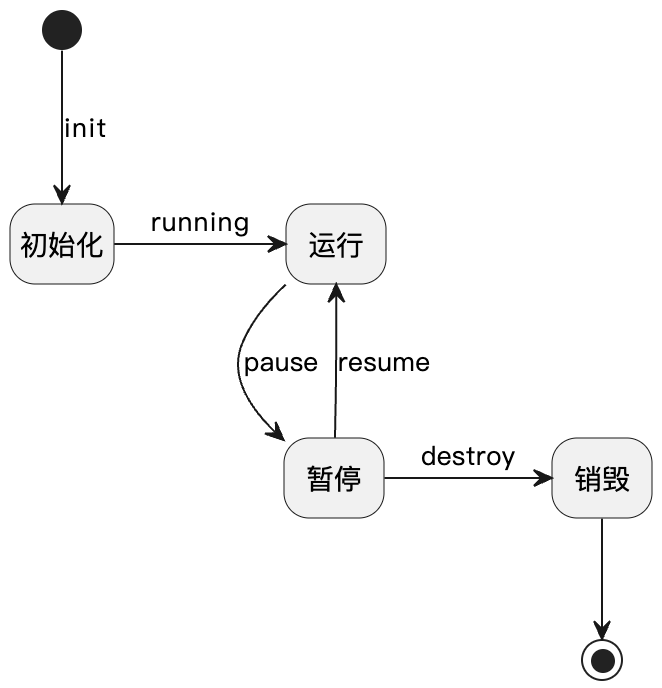
\includegraphics[width=0.45\textwidth]{task_status_gaiyao.png}
  \caption{任务模块状态机}
  \label{task_status_gaiyao}
\end{figure}

\section{调度模块概要设计}
调度模块的功能是根据调度策略控制任务模块的运行,调度模块唯一存在于每个不同的进程。调度模块根据用户提供的调度
配置文件创建调度任务并执行调度任务,调度配置文件如表\ref{schedule_config_file}所示。taks\_name是不同调度任务的名称,不同的调度任务
以任务名称区分;task\_callback是调度任务对应的回调函数,当任务被调度时将执行该函数。配置文件中的字段全部由
用户指定。
\begin{table}[H]
  \centering\small
  \caption{调度配置文件}
  \label{schedule_config_file}
  \begin{tabular}{cc}
    \toprule
    字段名 & 字段解释 \\
    \midrule
    task\_name & 调度任务名称\\
    task\_callback & 调度任务对应的回调函数\\
    \bottomrule
  \end{tabular}
\end{table}

调度模块的接口设计如表\ref{schedule_interface}所示。create\_message\_task接口用于创建基于消息触发的调度任务,create\_time\_task
接口用于创建基于时间触发的调度任务,avtivate\_task接口用于激活指定的调度任务。
\begin{table}[H]
  \centering\small
  \caption{调度模块接口设计}
  \label{schedule_interface}
  \begin{tabular}{cc}
    \toprule
    接口签名 & 接口解释 \\
    \midrule
    create\_message\_task & 创建基于消息触发的调度任务 \\
    create\_time\_task & 创建基于时间触发的调度任务 \\
    activate\_task & 激活指定调度任务 \\
    \bottomrule
  \end{tabular}
\end{table}

调度模块支持基于消息触发的调度策略和基于时间触发的调度策略。基于消息触发的调度策略是侵入式的,即该调度策略
并不需要由用户手动去激活调度任务,而是由通信抽象模块监听到新消息时调用订阅者模块中的回调函数,并最终在订阅者模块
的回调函数中激活对应调度任务。在同一个任务中,基于消息触发的调度任务数量等于订阅者数量。基于消息触发的调度策略
时序设计如图\ref{message_tick_gaiyao_sequence}所示。
\begin{figure}[H]
  \centering
  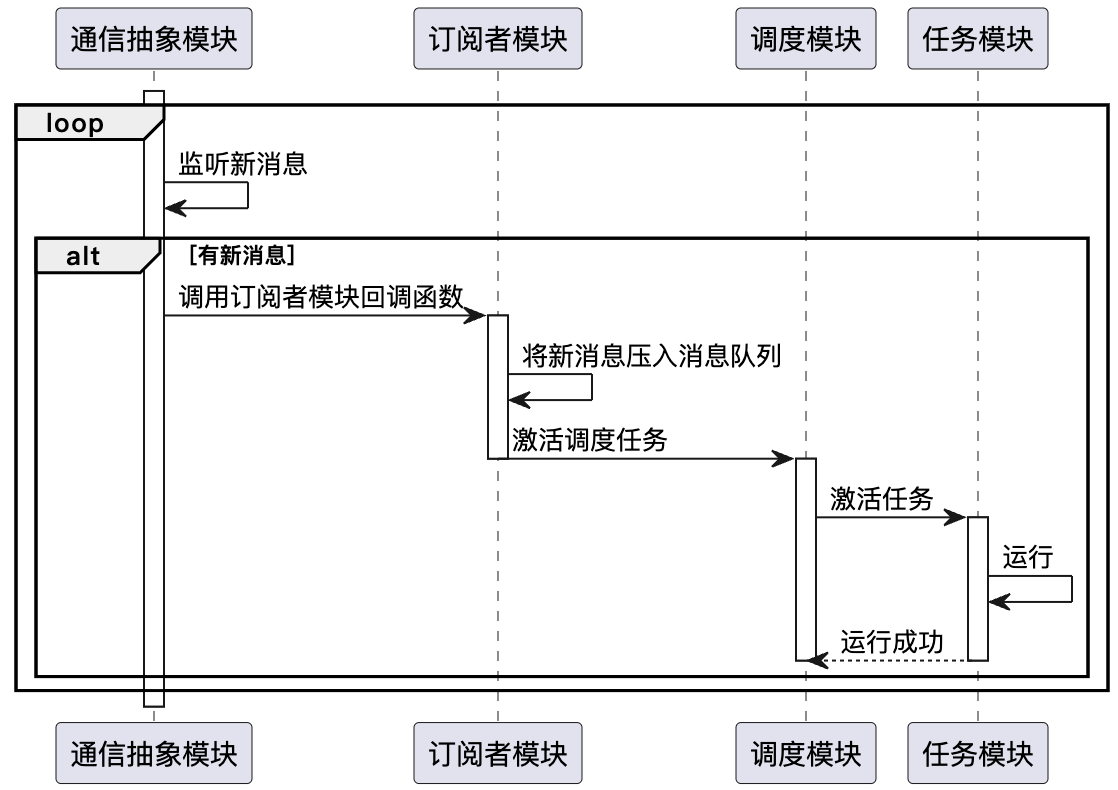
\includegraphics[width=0.9\textwidth]{message_tick_gaiyao_sequence.png}
  \caption{基于消息触发的调度策略时序图}
  \label{message_tick_gaiyao_sequence}
\end{figure}

基于时间触发的调度策略相较于基于消息触发调度策略不再是侵入式的,需要用户显式指定任务的调度频率。基于时间触发的调度策略
并不根据是否有新消息到来判断是否激活调度任务,而是从创建调度线程时就以固定的频率调用任务用户任务中的运行接口。该调度策略下,
调度模块记录首先计算任务在调度频率下的执行时间间隔,每当任务调度完成后继续计算当前时间与执行时间间隔计算调度剩余时间,
若调度剩余时间大于零,则在线程内睡眠剩余时间后再进行下一次调度,若调度剩余时间小于零,则立即进行下一次调度。基于时间触发的调度策略
时序设计如图\ref{time_tick_gaiyao_sequence}所示。
\begin{figure}[H]
  \centering
  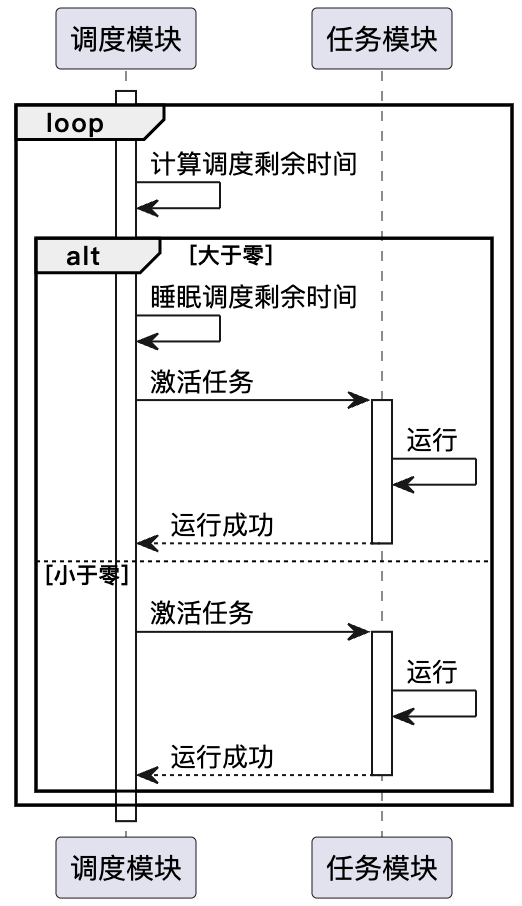
\includegraphics[width=0.4\textwidth]{time_tick_gaiyao_sequence.png}
  \caption{基于时间触发的调度策略时序图}
  \label{time_tick_gaiyao_sequence}
\end{figure}

\section{中心节点概要设计}
中心节点是本系统实现服务发现功能的核心模块,中心节点接受所有服务发现模块的RPC调用保存整个通信系统的网络拓扑信息并协助
各服务发现模块完成通信链路的建立。

\begin{figure}[htb]
  \centering
  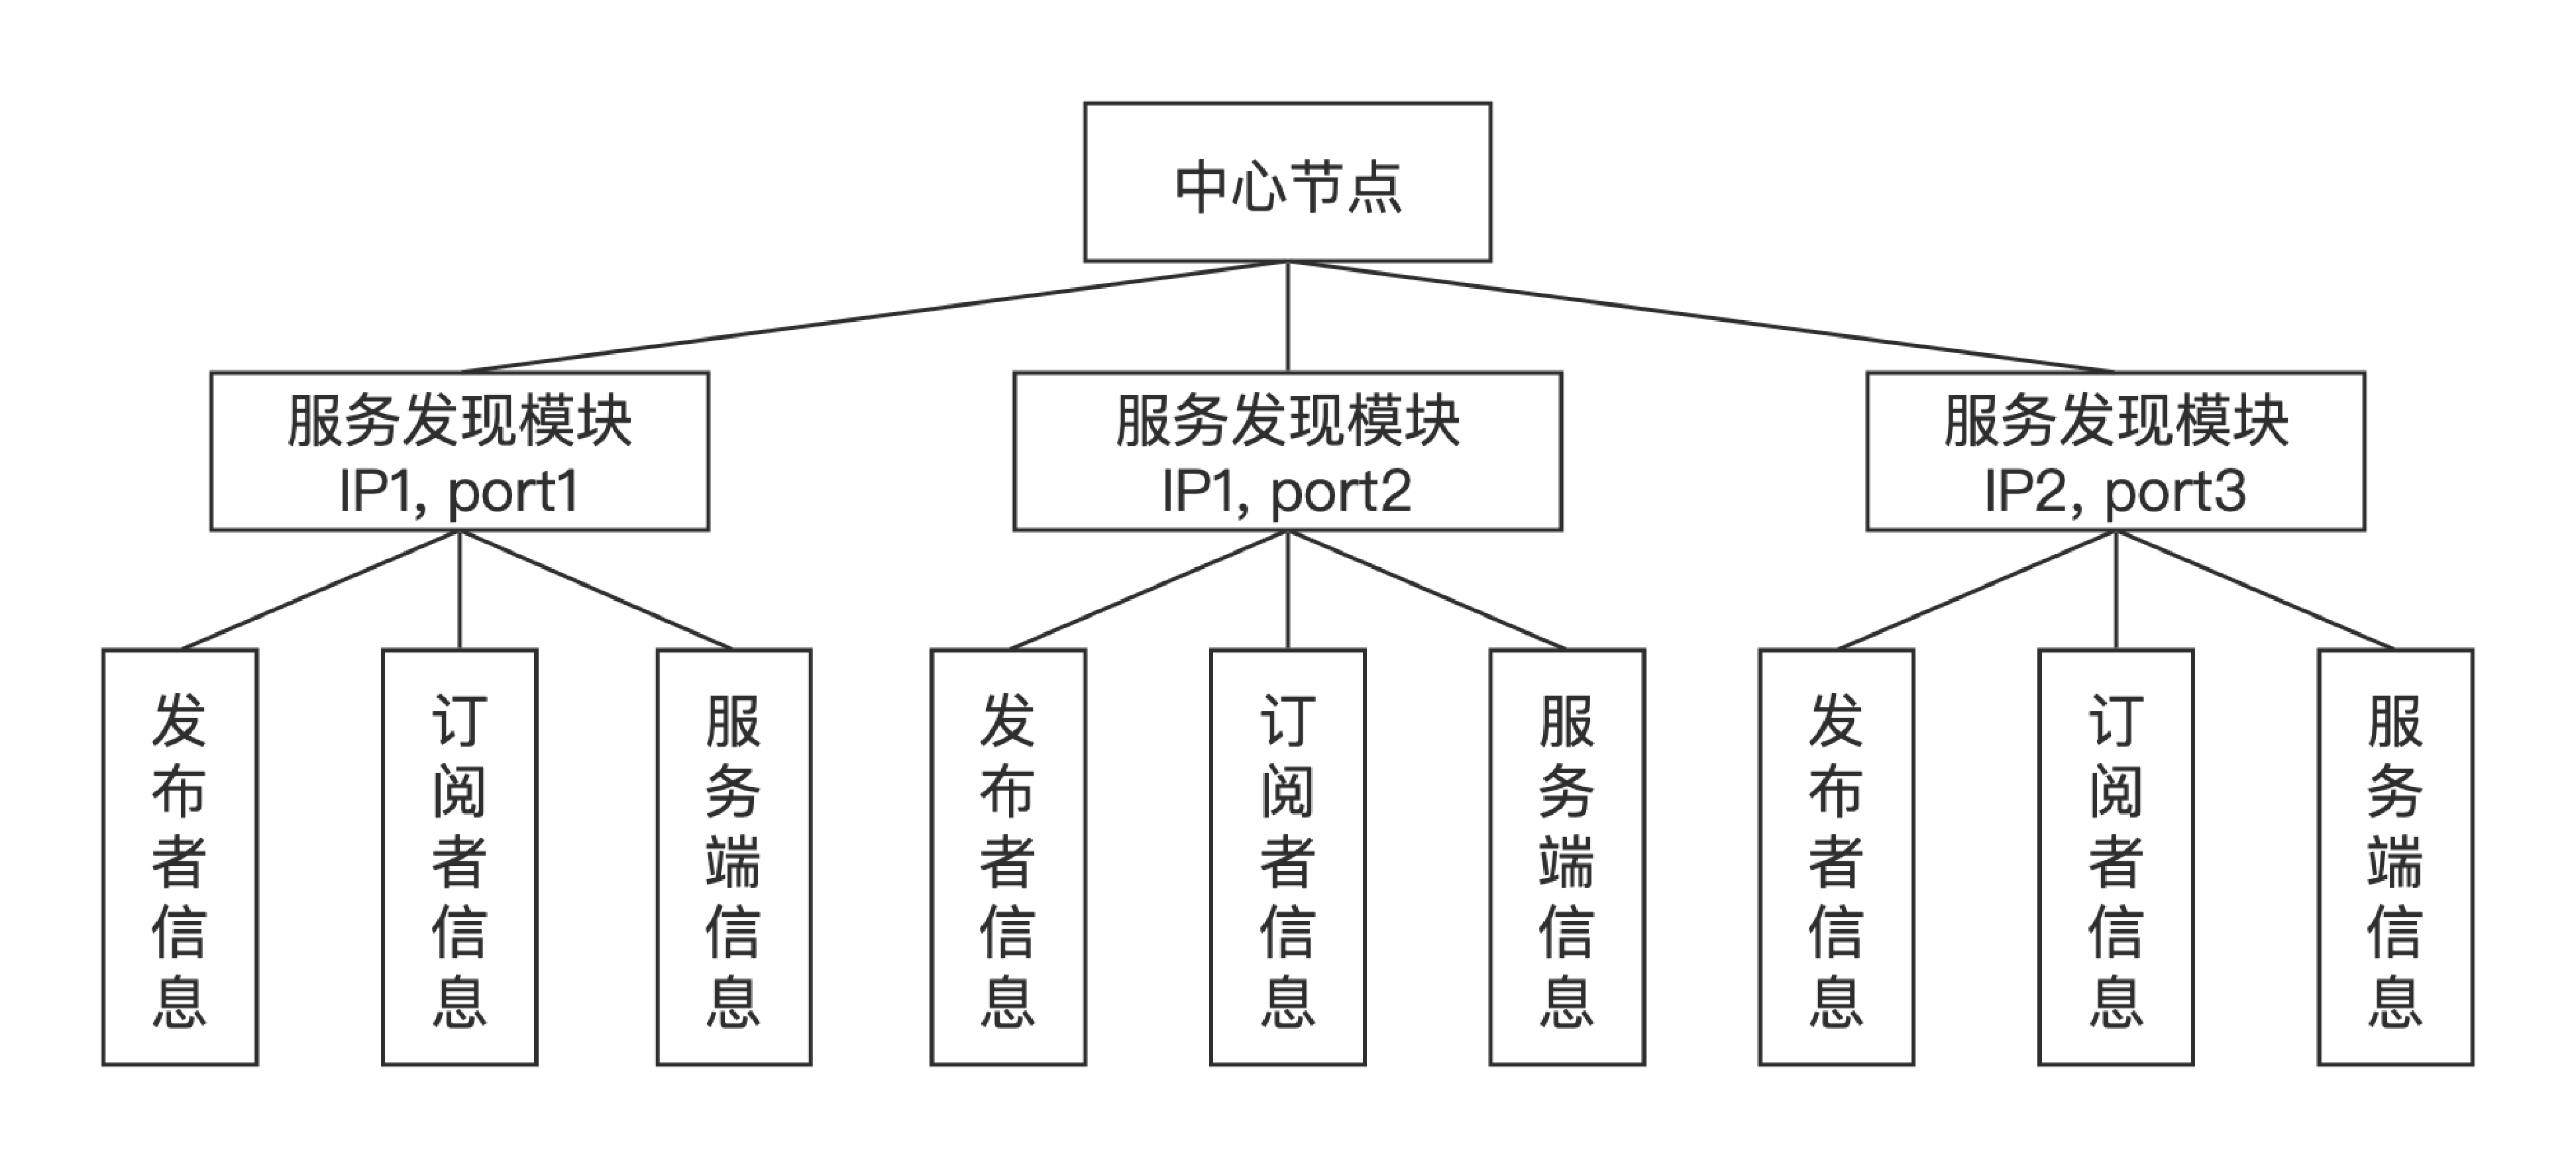
\includegraphics[width=0.9\textwidth]{storage_model.pdf}
  \caption{网络拓扑信息存储模型}
  \label{storage_model}
\end{figure}

中心节点根据IP地址以及端口号将服务发现模块进行区分,并且将每个服务发现模块中的网络拓扑信息进行单独存储,存储模型示意图如图\ref{storage_model}所示。
从图中可以看出,中心节点将IP地址与端口号两个信息中任意一个不相同的服务发现模块都进行区分。中心节点存储信息包括发布者信息、订阅者信息以及
服务端信息,三种信息都来自各服务发现模块进行主动发现时使用的请求参数。请求参数如\ref{service_discovery_parameter}中的PublisherInfo、SubscriberInfo和
ServiceServerInfo。

为了防止中心节点异常退出导致网络拓扑信息丢失,中心节点会定期将自身保存的通信系统网络拓扑信息转换为json文件并保存至本地。
当中心节点异常退出并重启时首先加载json文件中的历史网络拓扑信息,可以有效恢复异常退出前的网络拓扑信息并继续工作。
为了实时监控中心节点的运行状态,本系统使用linux脚本作为中心节点进程的监控手段,通过脚本完成启动中心节点和重启
中心节点的工作,如图\ref{master_EM}所示。
\begin{figure}[htb]
  \centering
  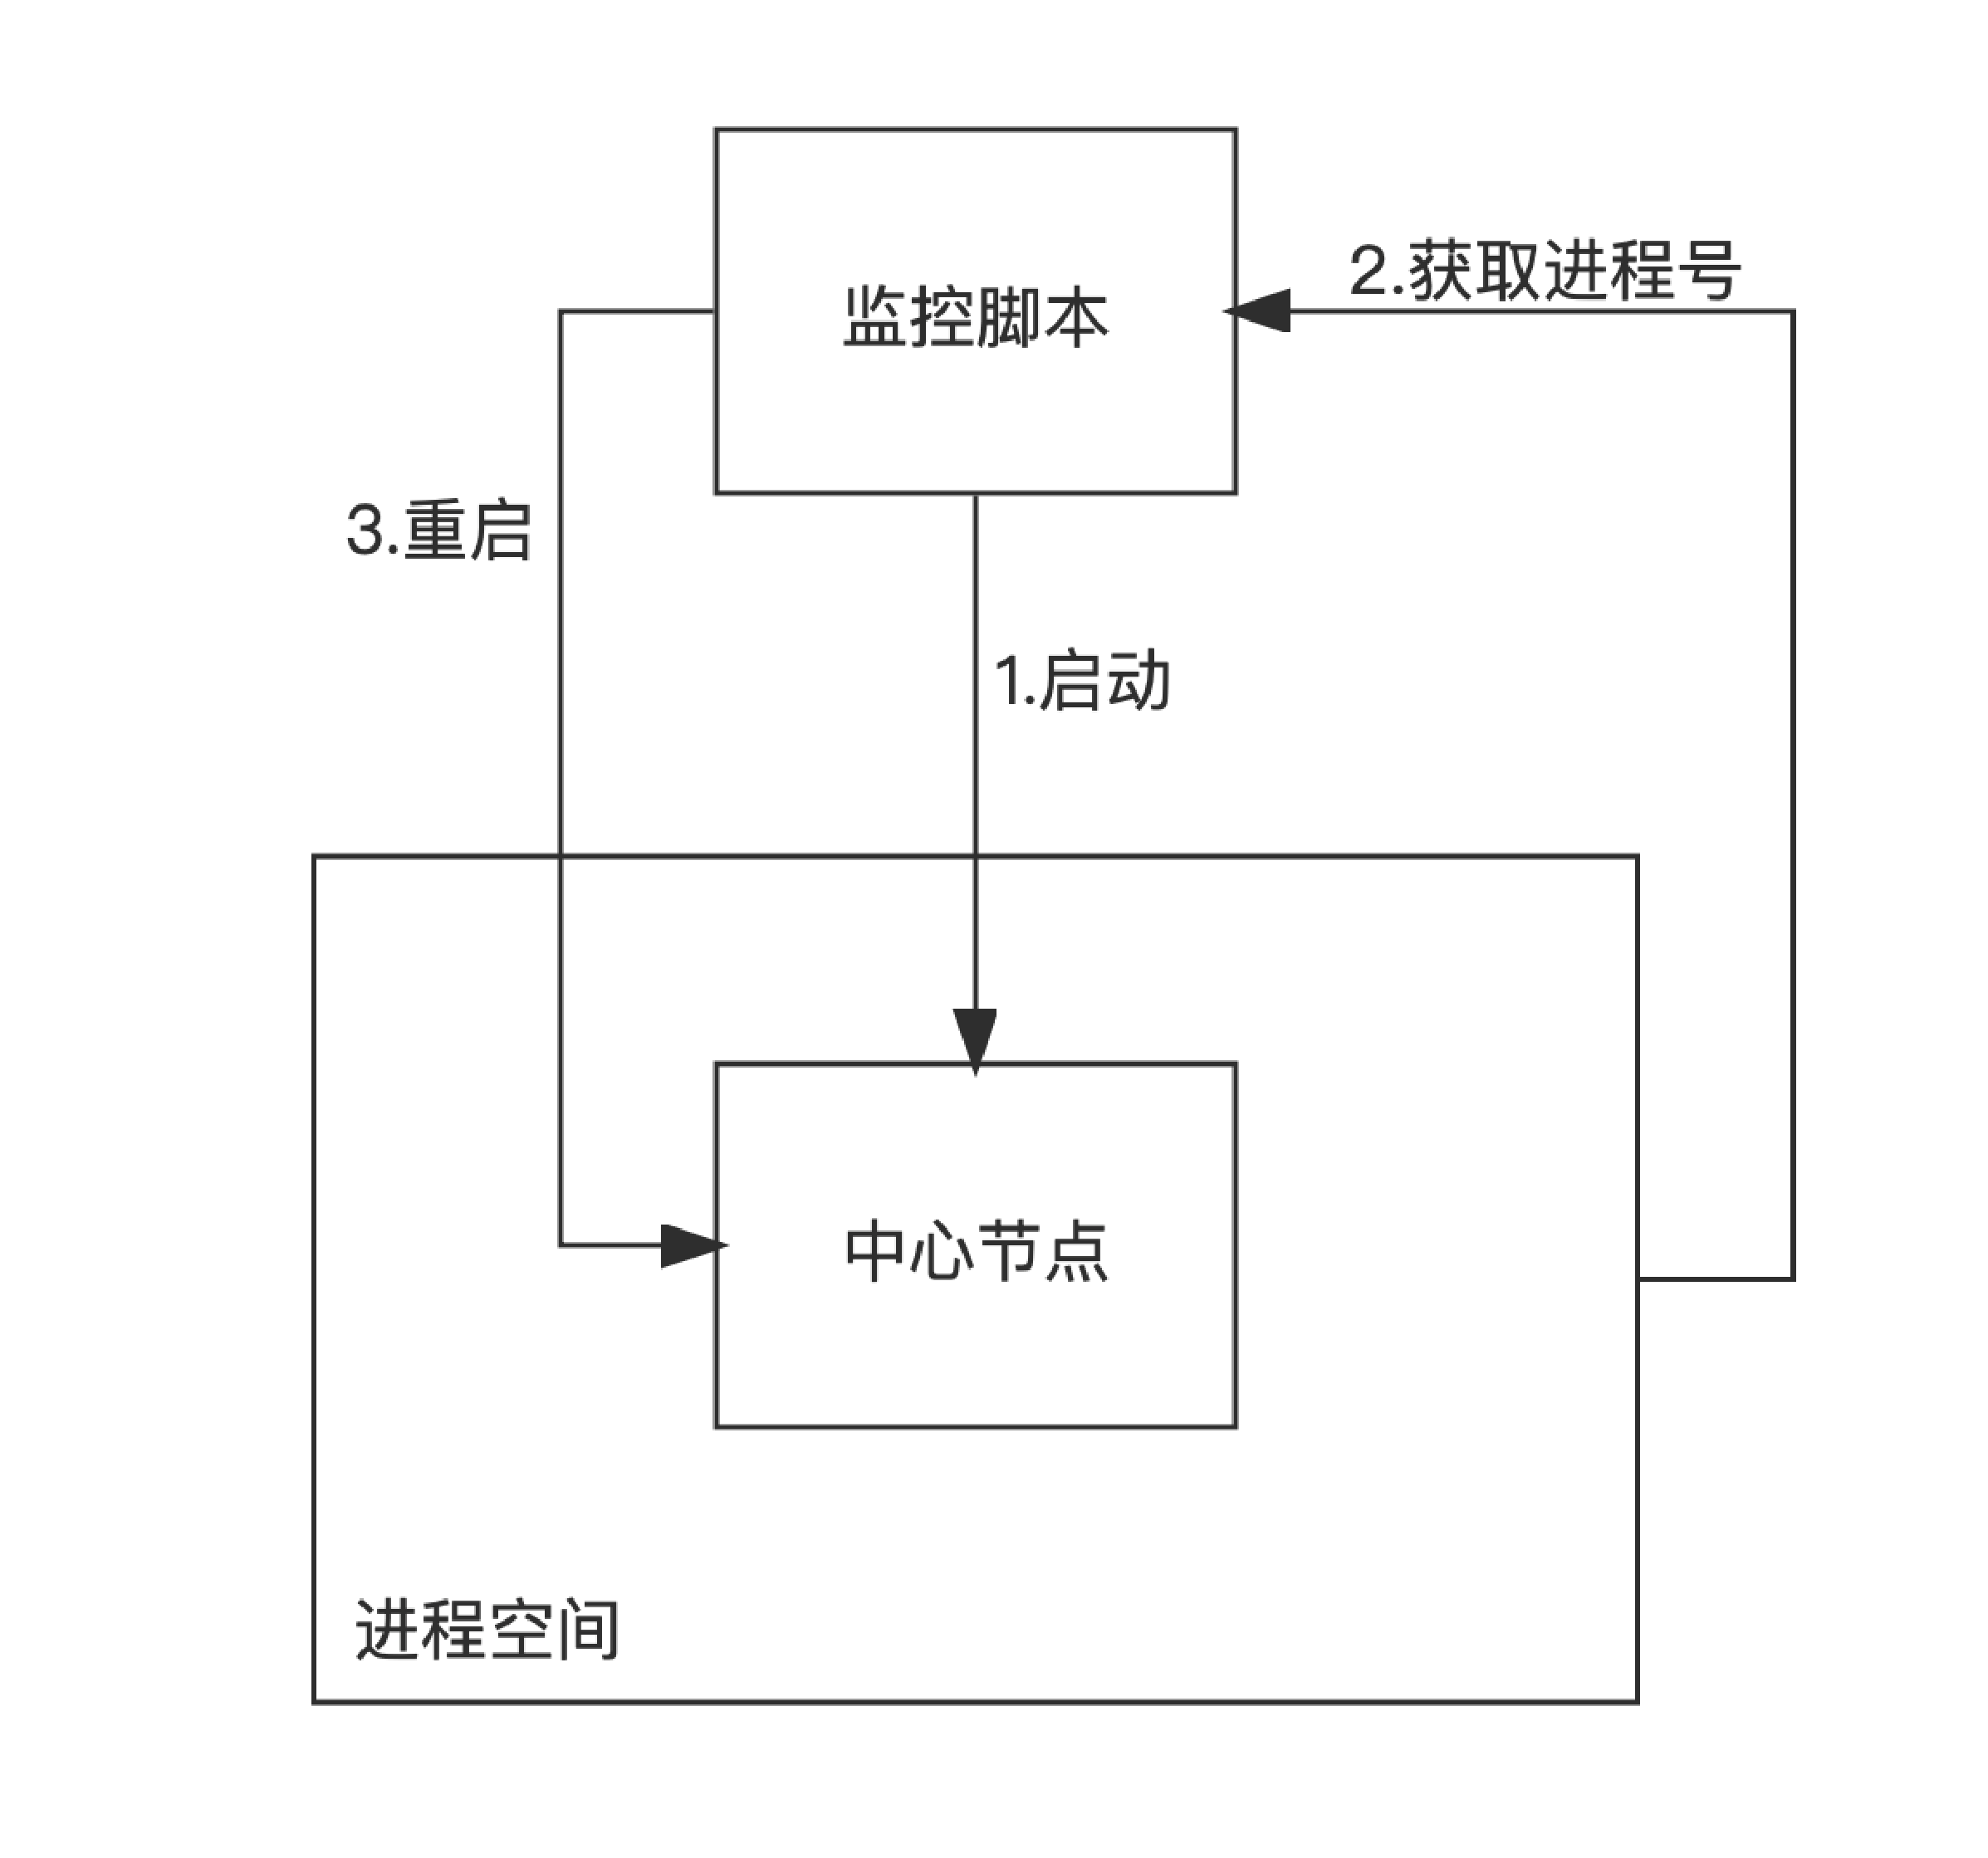
\includegraphics[width=0.6\textwidth]{master_EM.pdf}
  \caption{中心节点进程监控}
  \label{master_EM}
\end{figure}

中心节点提供了一系列供服务发现模块请求的服务,其中最主要的服务包括对发布者、订阅者以及服务端的注册、删除和修改。除此之外,中心节点
还提供网络拓扑信息查询服务。


\section{本章小结}
本章从自动驾驶运行时系统的整体结构为切入点,详细论述了该系统的整体结构;依次介绍系统各功能模块功能及设计思路、技术
重点和难点,为后续的详细设计与实现做铺垫。




